%%%%%%%%%%%%%%%%%%%%%%%%%%%%%%%%%%%%%%%%%
% Masters/Doctoral Thesis
% LaTeX Template
% Version 2.5 (27/8/17)
%
% This template was downloaded from:
% http://www.LaTeXTemplates.com
%
% Version 2.x major modifications by:
% Vel (vel@latextemplates.com)
%
% This template is based on a template by:
% Steve Gunn (http://users.ecs.soton.ac.uk/srg/softwaretools/document/templates/)
% Sunil Patel (http://www.sunilpatel.co.uk/thesis-template/)
%
% Template license:
% CC BY-NC-SA 3.0 (http://creativecommons.org/licenses/by-nc-sa/3.0/)
%
%%%%%%%%%%%%%%%%%%%%%%%%%%%%%%%%%%%%%%%%%

%----------------------------------------------------------------------------------------
%	PACKAGES AND OTHER DOCUMENT CONFIGURATIONS
%----------------------------------------------------------------------------------------

\documentclass[
11pt, % The default document font size, options: 10pt, 11pt, 12pt
%oneside, % Two side (alternating margins) for binding by default, uncomment to switch to one side
english, % ngerman for German
onehalfspacing, % Single line spacing, alternatives:  or doublespacing, singlespacing
%draft, % Uncomment to enable draft mode (no pictures, no links, overfull hboxes indicated)
%nolistspacing, % If the document is onehalfspacing or doublespacing, uncomment this to set spacing in lists to single
%liststotoc, % Uncomment to add the list of figures/tables/etc to the table of contents
%toctotoc, % Uncomment to add the main table of contents to the table of contents
%parskip, % Uncomment to add space between paragraphs
%nohyperref, % Uncomment to not load the hyperref package
headsepline, % Uncomment to get a line under the header
%chapterinoneline, % Uncomment to place the chapter title next to the number on one line
%consistentlayout, % Uncomment to change the layout of the declaration, abstract and acknowledgements pages to match the default layout
]{MastersDoctoralThesis} % The class file specifying the document structure

\usepackage[utf8]{inputenc} % Required for inputting international characters
%\usepackage[T1]{fontenc} % Output font encoding for international characters

\usepackage{mathpazo} % Use the Palatino font by default
\usepackage{amssymb}
\usepackage{amsfonts}
\usepackage{mathrsfs}
\usepackage{amsmath}
\usepackage{amsthm}
\usepackage{times}
\usepackage{graphicx}
\usepackage{enumitem}
\usepackage{hyperref}
\usepackage{setspace}
\usepackage{subcaption}
\usepackage{mathtools}

\usepackage[backend=bibtex,style=authoryear,natbib=true,doi=false,eprint=false,url=false,isbn=false]{biblatex} % Use the bibtex backend with the authoryear citation style (which resembles APA)

\addbibresource{phd_bibliography.bib} % The filename of the bibliography

\usepackage[autostyle=true]{csquotes} % Required to generate language-dependent quotes in the bibliography

\usepackage{lineno}
\linenumbers
\renewcommand{\baselinestretch}{1.5}

\newcommand{\diff}[2]{\frac{d #1}{d #2}}% to be used in mathmode
\newcommand{\cov}{\text{cov}} %to be used in mathmode
\newcommand{\var}{\text{var}} %to be used in mathmode

%----------------------------------------------------------------------------------------
%	MARGIN SETTINGS
%----------------------------------------------------------------------------------------

\geometry{
	paper=a4paper, % Change to letterpaper for US letter
	inner=2.5cm, % Inner margin
	outer=3.8cm, % Outer margin
	bindingoffset=.5cm, % Binding offset
	top=1.5cm, % Top margin
	bottom=1.5cm, % Bottom margin
	%showframe, % Uncomment to show how the type block is set on the page
}

%----------------------------------------------------------------------------------------
%	THESIS INFORMATION
%----------------------------------------------------------------------------------------

\thesistitle{Investigating, implementing, and creating methods for analysing large neuronal ensembles} % Your thesis title, this is used in the title and abstract, print it elsewhere with \ttitle
\supervisor{Dr. Cian \textsc{O'Donnell} \\
						Dr. Michael C. \textsc{Ashby}} % Your supervisor's name, this is used in the title page, print it elsewhere with \supname
\examiner{} % Your examiner's name, this is not currently used anywhere in the template, print it elsewhere with \examname
\degree{Doctor of Philosophy} % Your degree name, this is used in the title page and abstract, print it elsewhere with \degreename
\author{Thomas J. \textsc{Delaney}} % Your name, this is used in the title page and abstract, print it elsewhere with \authorname
\addresses{} % Your address, this is not currently used anywhere in the template, print it elsewhere with \addressname

\subject{Computer Science} % Your subject area, this is not currently used anywhere in the template, print it elsewhere with \subjectname
\keywords{} % Keywords for your thesis, this is not currently used anywhere in the template, print it elsewhere with \keywordnames
\university{\href{http://www.university.com}{University of Bristol}} % Your university's name and URL, this is used in the title page and abstract, print it elsewhere with \univname
\department{\href{http://department.university.com}{Department of Computer Science}} % Your department's name and URL, this is used in the title page and abstract, print it elsewhere with \deptname
\group{\href{http://researchgroup.university.com}{Biological Intelligence \& Machine Learning Unit}} % Your research group's name and URL, this is used in the title page, print it elsewhere with \groupname
\faculty{\href{http://faculty.university.com}{Engineering}} % Your faculty's name and URL, this is used in the title page and abstract, print it elsewhere with \facname

\AtBeginDocument{
\hypersetup{pdftitle=\ttitle} % Set the PDF's title to your title
\hypersetup{pdfauthor=\authorname} % Set the PDF's author to your name
\hypersetup{pdfkeywords=\keywordnames} % Set the PDF's keywords to your keywords
}

\begin{document}

\frontmatter % Use roman page numbering style (i, ii, iii, iv...) for the pre-content pages

\pagestyle{plain} % Default to the plain heading style until the thesis style is called for the body content

%----------------------------------------------------------------------------------------
%	TITLE PAGE
%----------------------------------------------------------------------------------------

\begin{titlepage}
\begin{center}

\vspace*{.06\textheight}
{\scshape\LARGE \univname\par}\vspace{1.5cm} % University name
\textsc{\Large Doctoral Thesis}\\[0.5cm] % Thesis type

\HRule \\[0.4cm] % Horizontal line
{\huge \bfseries \ttitle\par}\vspace{0.4cm} % Thesis title
\HRule \\[1.5cm] % Horizontal line

\begin{minipage}[t]{0.4\textwidth}
\begin{flushleft} \large
\emph{Author:}\\
\authorname % Author name - remove the \href bracket to remove the link
\end{flushleft}
\end{minipage}
\begin{minipage}[t]{0.4\textwidth}
\begin{flushright} \large
\emph{Supervisors:} \\
\supname % Supervisor name - remove the \href bracket to remove the link
\end{flushright}
\end{minipage}\\[2cm]

\vfill

\large \textit{A thesis submitted in fulfillment of the requirements\\ for the degree of \degreename}\\[0.3cm] % University requirement text
\textit{in the}\\[0.4cm]
\groupname\\\deptname\\[1cm] % Research group name and department name


{\large \today} % Date
%\includegraphics{Logo} % University/department logo - uncomment to place it
\begin{flushright}
Word count: $39000$ \\[4cm]
\end{flushright}
\vfill
\end{center}
\end{titlepage}

%----------------------------------------------------------------------------------------
%	DECLARATION PAGE
%----------------------------------------------------------------------------------------


\begin{declaration}
\addchaptertocentry{\authorshipname} % Add the declaration to the table of contents
% \noindent I, \authorname, declare that this thesis titled, \enquote{\ttitle} and the work presented in it are my own. I confirm that:
%
% \begin{itemize}
% \item This work was done wholly or mainly while in candidature for a research degree at this University.
% \item Where any part of this thesis has previously been submitted for a degree or any other qualification at this University or any other institution, this has been clearly stated.
% \item Where I have consulted the published work of others, this is always clearly attributed.
% \item Where I have quoted from the work of others, the source is always given. With the exception of such quotations, this thesis is entirely my own work.
% \item I have acknowledged all main sources of help.
% \item Where the thesis is based on work done by myself jointly with others, I have made clear exactly what was done by others and what I have contributed myself.\\
% \end{itemize}

I declare that the work in this dissertation was carried out in accordance with the requirements of the University's Regulations and Code of Practice for Research Degree Programmes and that it has not been submitted for any other academic award. Except where indicated by specific reference in the text, the work is the candidate's own work. Work done in collaboration with, or with the assistance of, others, is indicated as such. Any views expressed in the dissertation are those of the author.

\noindent Signed:\\
\rule[0.5em]{25em}{0.5pt} % This prints a line for the signature

\noindent Date:\\
\rule[0.5em]{25em}{0.5pt} % This prints a line to write the date
\end{declaration}

\cleardoublepage

%----------------------------------------------------------------------------------------
%	QUOTATION PAGE
%----------------------------------------------------------------------------------------

% \vspace*{0.2\textheight}
%
% \noindent\enquote{\itshape Thanks to my solid academic training, today I can write hundreds of words on virtually any topic without possessing a shred of information, which is how I got a good job in journalism.}\bigbreak
%
% \hfill Dave Barry

%----------------------------------------------------------------------------------------
%	ABSTRACT PAGE
%----------------------------------------------------------------------------------------

\begin{abstract}
\addchaptertocentry{\abstractname} % Add the abstract to the table of contents

Since the use of multi-electrode recording in neuroscience began, the number neurons being recorded in parallel has been increasing. Recently developed methods using calcium or voltage imaging have also contributed to the growth in neuronal datasets. As datasets grow, the need for new analysis methods also grows. In this research we attempted to address some of the problems associated with reading from large neuronal ensembles using fluorescent calcium indicators, and some of the problems with analysing data read from large neuronal ensembles.

We created a biophysical model for the fluorescence trace produced by a calcium indicator responding to a given spike train. Our model reproduced the characteristics of a real fluorescence trace recognised by spike inference algorithms. This model will be useful for anyone using or considering calcium imaging.

To find order in the correlated behaviour of a large mutli-region neuronal ensemble, we applied a novel method from network science to detect structure and communities in correlated behaviour. We investigated the similarities between these communities and their brain anatomy. Our results indicate local correlated networks function at shorter timescales ($<50$ms), while mutli-region correlated networks function over longer timescales ($>100$ms). This result agrees with previous findings from EEG data, but has not been shown before using spiking data.

We developed a statistical model for the number of neurons spiking in a neuronal ensemble based on the Conway-Maxwell-binomial distribution. Our aim was to capture correlated activity in a neuronal population without measuring correlation coefficients directly. The model captured correlated activity at very short timescales better than measuring correlation coefficients. We also replicated one of the findings of Churchland et al. (2010) relating to the quenching of neural variability at stimulus onset. We propose a connection between this result and the changes in association captured by our model.

\end{abstract}

%----------------------------------------------------------------------------------------
%	ACKNOWLEDGEMENTS
%----------------------------------------------------------------------------------------

\begin{acknowledgements}
\addchaptertocentry{\acknowledgementname} % Add the acknowledgements to the table of contents
I would like to thank my supervisors, Cian O'Donnell and Mike Ashby, for their help, encouragement, advice, and patience over the last four years. This includes not only helping with research, but also enabling and encouraging me to make the most of my opportunities during that time. Without their help, I would not have grown as much as I have done in those years. I very grateful for their time and effort.

I would also like to thank the members of the Bristol Computational Neuroscience Unit for introducing me to all the various aspects of computer science, neuroscience, and machine learning, of which I otherwise would not have heard. As the first person to introduce me to the concept of mathematical neuroscience during my undergraduate days, and a great source of advice and guidance during my PhD, I would also like to thank Conor Houghton.

Personally, I would to thank my girlfriend Ashley, who has been nothing but helpful since I met her.

Finally, I would like to that my father, mother, brother and sister. I am truly fortunate to have such a good family. I thank them for their love, encouragement, and excellent example.
\end{acknowledgements}

%----------------------------------------------------------------------------------------
%	LIST OF CONTENTS/FIGURES/TABLES PAGES
%----------------------------------------------------------------------------------------

\tableofcontents % Prints the main table of contents

\listoffigures % Prints the list of figures

\listoftables % Prints the list of tables

%----------------------------------------------------------------------------------------
%	ABBREVIATIONS
%----------------------------------------------------------------------------------------

\begin{abbreviations}{ll} % Include a list of abbreviations (a table of two columns)

\textbf{COMb} & Conway-Maxwell-binomial (distribution) \\
\textbf{OASIS} & Online active set method to infer spikes \\
\textbf{SNR} & Signal to noise ratio \\

\end{abbreviations}

%----------------------------------------------------------------------------------------
%	PHYSICAL CONSTANTS/OTHER DEFINITIONS
%----------------------------------------------------------------------------------------

% \begin{constants}{lr@{${}={}$}l} % The list of physical constants is a three column table
%
% % The \SI{}{} command is provided by the siunitx package, see its documentation for instructions on how to use it
%
% Speed of Light & $c_{0}$ & \SI{2.99792458e8}{\meter\per\second} (exact)\\
% %Constant Name & $Symbol$ & $Constant Value$ with units\\
%
% \end{constants}

%----------------------------------------------------------------------------------------
%	SYMBOLS
%----------------------------------------------------------------------------------------

\begin{symbols}{lll} % Include a list of Symbols (a three column table)

$[Ca^{2+}]$ & Free calcium concentration & \si{\mole} \\
$[BCa]$ & Fluorescent indicator bound calcium & \si{\mole} \\
$[ECa]$ & Endogenous mobile buffer bound calcium & \si{\mole} \\
$[ImCa]$ & Immobile mobile buffer bound calcium & \si{\mole} \\
$[BCa^{\ast}]$ & excited fluorescent indicator bound calcium & \si{\mole} \\
$k_{X_f}$ & binding (affinity) rate & \si{\per\mole \per\second} \\
$k_{X_b}$ & unbinding (dissociation) rate & \si{\per\second} \\
%Symbol & Name & Unit \\

% \addlinespace % Gap to separate the Roman symbols from the Greek

% $\omega$ & angular frequency & \si{\radian} \\

\end{symbols}

%----------------------------------------------------------------------------------------
%	DEDICATION
%----------------------------------------------------------------------------------------

%\dedicatory{For/Dedicated to/To my\ldots}

%----------------------------------------------------------------------------------------
%	THESIS CONTENT - CHAPTERS
%----------------------------------------------------------------------------------------

\mainmatter % Begin numeric (1,2,3...) page numbering

\pagestyle{thesis} % Return the page headers back to the "thesis" style

% Include the chapters of the thesis as separate files from the Chapters folder
% Uncomment the lines as you write the chapters

\chapter{Introduction}

\label{chap:intro}

\section{Overview}
% Ideas (not in order):
% \begin{itemize}
%     \item From small to big datasets (in terms of number of neurons)
%     \item Big datasets mean statistical methods are more necessary (curse of dimensionality)
%     \item Big datasets mean higher order correlations are more meaningful (schneidman)
%     \item Exploit pairwise correlations in different way (eight probe)
%     \item abandon correlations embrace association (COMB)
%     \item electrophysiology drawbacks vs calcium benefits
%     \item calcium drawbacks (fluorescence modelling) (mention nuclear filling and cell pathology) (mention that calcium imaging can only be used near the surface of the brain, e-phys can go deeper, especially with new probes)
% \end{itemize}

Since Hodgkin and Huxley's squid experiments featuring a single axon \parencite{hodgkin}, to more recent research with spike sorted data from  $\sim 24000$ neurons from $34$ brain regions from $21$ mice \parencite{allen}, the number of neurons contributing to electrophysiological datasets has been growing. Recording methods using two-photon calcium imaging have also been used to extract data from populations containing over $10000$ neurons \parencite{peron}. This dramatic growth in the number of neurons available for analysis requires a dramatic change in analysis methods. In this project, we have attempted to address some of the difficulties in collecting data from these large ensembles, and analysing these data.

To focus on calcium imaging for a start, a neuron that contains a fluorescent calcium indicator in its cytoplasm will fluoresce when bombarded with photons. The amount that the cell will fluoresce is dependent on the concentration of fluorescent indicator within the cell, and the concentration of calcium within the cell. When a neuron fires an action potential, the influx of free calcium ions causes an increase in fluorescence when those ions bond with the fluorescent indicator and those bounded molecules are bombarded with photons. After the action potential, as calcium is extruded from the cell the fluorescence returns to a baseline level. This is the basic mechanism of fluorescent calcium indicator based imaging.

This method has some advantages over electrophysiology as measure of neuronal ensemble activity. Isolating individual neurons is easier and more reliable than identifying unique spike sources in electrophysiology \parencite{buccino}. Also, spike sorting methods can only detect spikes, but imaging methods can also detect cells that are not spiking, because cells will emit a baseline level of fluorescence when not firing action potentials. Calcium imaging sites can be re-used for weeks for longitudinal studies \parencite{chen}. The fluorescent indicator is delivered to the cell by adeno-associated viruses, consequently there can be problems with indicator gradients around the infection site, and expression levels will change in individual cells over weeks \parencite{tian, chen}. This delivery method can also cause cell pathology, and nuclear filling \parencite{zariwala}, but these problems can be solved by using lines of transgenic mice \parencite{dana}. The fluorescence signal itself can serve a a good indicator of cell activity, but similarly to electrophysiology, the aim of calcium imaging is often spike detection.

If the imaging data is collected at a high enough frequency, and the signal-to-noise ratio of the fluorescence trace is high enough, it should be possible to infer the spike times to some level of accuracy. For example, the calmodulin based indicator GCaMP6s has a sufficiently high signal-to-noise ratio that isolated action potentials can be detected and inferred \parencite{chen}. Many spike inference algorithms exist \parencite{vogelstein, pnevmatikakis, friedrich, paninski1, paninski2, deneux, greenberg}, and some of these can perform both cell isolation and spike detection simultaneously \parencite{vogelstein, pnevmatikakis, paninski2, deneux}. But the relationship between spiking and fluorescence change is not fully understood. For example, the fluorescent indicator will act like an additional calcium buffer within the cell cytoplasm and will compete with the other endogenous buffers to bind with free calcium cells. Therefore, the concentration of those endogenous buffers, and the binding dynamics of those buffers will have an effect on the change in fluorescence in response to an action potential. Furthermore, the binding dynamics of the fluorescent indicator itself will have an effect on the change in fluorescence. For example, the GCaMP series of fluorescence indicators are based on the calcium buffer protein \texttt{calmodulin}. This protein has four binding sites, whose affinities interact non-linearly. But most of the spike inference algorithms model the fluorescence as a linear function of a calcium trace, and they model this calcium trace as a first or second order autoregression with a pulse input to represent action potentials. Deneux et al. (2016) developed a spike inference algorithm with a bit more biological inspiration, but this amounted to a very similar process. While this autoregression idea appears to be a reasonable approximation, the algorithms that use this approximation are outperformed by the most recently published spike inference algorithm to be cited here \parencite{greenberg}. This algorithm does take into account the binding dynamics of both the endogenous buffers and fluorescent calcium indicator, and the concentrations of free calcium, indicator, and endogenous buffer within the cell cytoplasm. This shows that there is value in more biologically inspired models of fluorescent calcium indicators.

In light of the growing popularity of two-photon calcium imaging, and the lack of biologically inspired spike inference algorithms (Greenberg et al. developed their spike inference algorithm in parallel to our work), we decided to develop a biologically inspired model for fluorescent calcium indicator fluorescence. The idea being that our model would take a spike train, or simply spike times, provided by the user, and return the fluorescence trace that would be induced by this spike train or spike times. The model contains parameters for concentrations of indicator and endogenous buffers, as well as affinity and unbinding rates for these buffers. There are also parameters for the baseline concentration of free calcium in the cell cytoplasm, and the cell radius (as a means for calculating the cell volume). With this model, we hoped that experimentalists would be able to test out different calcium indicators on the types of spike trains that they expect to encounter. This way they could decide ahead of time which indicator suited their situation best. Since the output of our model is a fluorescence trace, the spike inference models mentioned above can be applied to the modelled fluorescence. This means that the model could also be used to benchmark the performance of these spike inference algorithms, and to investigate the impact of variations in the model on spike inference accuracy.

We have outlined some of the advantages that calcium imaging has over electrophysiology. But electrophysiology is more useful in some situations. One particular drawback for two-photon calcium imaging is that it can only be used for imaging near to the surface of the brain. Although imaging with three (or presumably more) photons may solve this problem in the future \parencite{ouzounov}. A better option for reading activity from neurons beyond the surface of the brain is to use Neuropixels probes \parencite{jun}. These probes can be used to read from thousands of neurons simultaneously in many different areas of the brain \parencite{allen, stringer, steinmetz, steinmetz2019}. This brings us to another problem for which we require new innovations in our analysis methods. Specifically, analysing correlated behaviour in neural ensembles consisting of neurons from many different brain regions.

Until the invention of new technologies such as the Neuropixels probes, most electrophysiology datasets read from neurons in only one or two regions. Therefore most of the research on interactions between neurons in different regions is limited to two regions \parencite{wierzynski, patterson, girard}. In chapters \ref{chap:eight_probe} and \ref{chap:comb} we used datasets with neurons from $9$ and $5$ different brain regions respectively.

% might be asked to expand this paragraph, could explain more about the findingings in the citations.

In light of recent findings based on correlated behaviour showing that spontaneous behaviours explain activity in many different parts of the brain that would otherwise be regarded as noise \parencite{stringer}, that satiety is represented brain wide \parencite{allen}, and that exploratory and non-exploratory states are represented in the amygdala \parencite{grundemann}, it was clear that state representation or motor control had an influence on correlated behaviour in areas of the brain not usually associated with these tasks. Also, given differences in timescales of fluctuations in different brain regions \parencite{murray}, and different timescales for event representation in different brain regions \parencite{baldassano}, we decided to investigate brain wide correlated behaviour at timescales ranging from $5$ms up to $3$s.

We started off measuring the correlations in spike counts between individual neurons in our ensemble. These measurements induced a weighted undirected graph where each node represented a neuron, and the weight of each edge was the strength of the correlation between the neurons represented by the nodes at either end of that edge. In order to put the neurons into groups with correlated behaviour, we applied a novel community detection algorithm \parencite{humphries} to this graph. We repeated this analysis for timescales from milliseconds to seconds. Bear in mind that our correlation based graph was completely agnostic of the anatomical regions in which our cells resided. We then compared our correlated communities to their anatomy at each timescale. In this way, we used a novel method, never applied neuronal data before, to analyse the makeup of correlated communities across different regions at different timescales.

Many important findings have been made by measuring the correlations between binned spike counts, but there are some problems with this method of analysis. Firstly, the width of the bins used to bin spike times into spike counts has an effect on the magnitude of the correlations measured. Using a short bin width can cause your measurements to be artificially small \parencite{cohen2}. This may not be an issue if one is considering relative size of correlations when using the same bin width, but it is still not ideal. Secondly, while pairwise correlations can capture most of the information in a small network (up to $40$ cells) of highly correlated cells \parencite{schneidman}, a model based on pairwise correlations alone will fail to capture the activity of larger ($\sim 100$ cells) networks, higher order correlated activity is required \parencite{ganmor}. One problem with these higher order correlations is that they may be defined in different ways \parencite{staude}. Furthermore if we want to include them in a model this usually involves greatly increasing the number of parameters to fit, which increases the dimension of the parameter space leading to the `curse of dimensionality'.
Some models attempt to sidestep these problems while still capturing higher-order correlations. These models attempt to capture the relationship between each individual neuron in the ensemble, and the ensemble as a whole. Okun et al (2015) called the strength of this relationship the `population coupling', and demonstrated that this quantity can predict an individual neuron's response to optogenetic stimulation of the whole ensemble. They also showed that this quantity was an indicator of the neuron's synaptic connectivity \parencite{okun}. With the `population tracking model', O'Donnell et al. (2016) linked the probability of firing an action potential for each individual neuron with the distribution of the number of active neurons. This allowed model fitting for a large number of neurons, as well as calculation of full pattern probabilities, and population entropy \parencite{odonnell}.

In this work, we also aimed to capture correlated behaviour between the neurons in a neuronal ensemble without measuring correlations directly. Correlation coefficients capture the linear component of the relationship between two random variables, but will not measure any relationship beyond linearity. Also, measuring correlation coefficients using short timebins can be difficult for neuronal data \parencite{cohen2}. We decided to abandon correlation, and we aimed to quantify a more general concept of association by modelling the number of active neurons in the ensemble using a Conway-Maxwell-binomial (COMb) distribution \parencite{kadane_2016}.

The COMb distribution is a probability distribution over the number of successes in a sequence of Bernoulli trials, where these trials can be associated in some way. The COMb distribution is an extension of the standard binomial distribution, with an additional parameter to model association between the Bernoulli variables. Using this additional parameter the distribution can capture positive association, where the Bernoulli variables tend to take the same value, negative association, where the Bernoulli variables tend to take opposite values, or no association i.e. the standard binomial distribution.

We fit a COMb distribution to spike sorted electrophysiological data taken from five different regions in the brain of an awake mouse exposed to visual stimuli \parencite{steinmetz2019}. We examined whether or not a model based on the COMb distribution was able to capture changes in the number of active neurons in these neuronal ensembles in response to the stimuli. We also investigated the relationship between the changes as captured by the COMb model and the change in neural variability as measured by Churchland et al. in their famous paper \parencite{Churchland}.

Our overall aim was to investigate some of the challenges in analysing large ensembles of neurons present today. That included collecting the data to analyse (via calcium imaging), and subsequently analysing these data. We felt that this was a worthwhile project because the size of datasets, in terms of numbers of neurons and data collected, is growing rapidly. Consequently these challenges will only become greater unless they are addressed. This is our attempt at addressing them.

\documentclass[a4paper,12pt]{article}
\usepackage[utf8x]{inputenc}
\usepackage{amssymb}
\usepackage{amsfonts}
\usepackage{mathrsfs}
\usepackage{amsmath}
\usepackage{amsthm}
\usepackage[margin=3cm]{geometry}
\usepackage{times}
\usepackage{graphicx}
\usepackage{enumitem}
\usepackage{fancyhdr}
\usepackage{hyperref}
\usepackage{setspace}
\usepackage{subcaption}
\usepackage{mathtools}

\pagestyle{fancy}
\fancyhf{}
\lhead{Thomas Delaney}
\rhead{Fluorescence Modelling}
\cfoot{\thepage}

\newtheorem{theorem}{Theorem}
\newtheorem{proposition}{Proposition}[section]
\newtheorem{lemma}{Lemma}[section]
\newtheorem{corollary}{Corollary}[section]
\theoremstyle{definition}
\newtheorem{definition}{Definition}[section]

\newcommand{\boldnabla}{\mbox{\boldmath$\nabla$}} % to be used in mathmode
\newcommand{\cbar}{\overline{\mathbb{C}}}% to be used in mathmode
\newcommand{\diff}[2]{\frac{d #1}{d #2}}% to be used in mathmode
\newcommand{\difff}[2]{\frac{d^2 #1}{d #2^2}}% to be used in mathmode
\newcommand{\pdiff}[2]{\frac{\partial #1}{\partial #2}} % to be used in mathmode
\newcommand{\pdifff}[2]{\frac{\partial^2 #1}{\partial #2^2}}% to be used in mathmode
\newcommand{\upperth}{$^{\mbox{\footnotesize{th}}}$}%to be used in text mode
\newcommand{\vect}[1]{\mathbf{#1}}% to be used in mathmode
\newcommand{\curl}[1]{\boldnabla \times \vect{#1}} % to be used in mathmode
\newcommand{\divr}[1]{\boldnabla \cdot \vect{#1}} %to be used in mathmode
\newcommand{\modu}[1]{\left| #1 \right|} %to be used in mathmode
\newcommand{\brak}[1]{\left( #1 \right)} % to be used in mathmode
\newcommand{\comm}[2]{\left[ #1 , #2 \right]} %to be used in mathmode
\newcommand{\dop}{\vect{d}} %to be used in mathmode
\newcommand{\cov}{\text{cov}} %to be used in mathmode
\newcommand{\var}{\text{var}} %to be used in mathmode
\newcommand{\mb}{\mathbf} %to be used in mathmode
\newcommand{\bs}{\boldsymbol} %to be used in mathmode
% Title Page
\title{Modelling the fluorescence produced by fluorescent calcium indicators in response to sequences of action potentials}
\date{}
\author{Thomas J. Delaney \\ Cian O'Donnell, Michael C. Ashby}

\begin{document}

\maketitle

\newpage

\abstract{The use of fluorescent calcium indicators, such as GCaMP6s, to monitor neuronal activity is widespread. But the relationship between the fluorescence signal and action potential firing is poorly understood. Furthermore, the effects of the indicator characteristics on this fluorescence signal are unknown. For example, it is known that genetically encoded indicators accumulate within neurons over weeks and months. This makes comparison of activity levels at different time points difficult. As a result, whether or not spike train inference is always possible using fluorescent calcium indicators remains unknown.

The aim of this project was to model the fluorescence traces produced by a fluorescent calcium indicator in a neuron soma, given parameters such as binding rate, dissociation rate, and molecular concentration from a specific spike train. The ultimate goal of the model is to allow benchmarking of the various spike inference algorithms that have been developed, and to understand how indicator characteristics affect the quality of spike train inference.

The modelled cell contents consisted of free calcium, fluorescent indicator molecules, and mobile and immobile endogenous calcium buffers. The indicator molecules which were bound to a calcium molecule could be either excited, i.e. able to release a photon, or relaxed. In order to reproduce the noise in the system dynamics, we modelled the release of photons from the excited indicator bound calcium as a stochastic process.

The fluorescence traces produced by the simulation were calibrated to reproduce the signal-to-noise ratio observed in experimental data. Spike inference algorithms were used to infer spike trains from the experimental fluorescence traces and the modelled fluorescence traces. The parameters of the model were then varied in order to determine the effect on the system dynamics and the effects on spike inference.} % no citations in the abstract

\newpage

\tableofcontents

\newpage

\section{Calcium Imaging}

\begin{figure}[p]
  \begin{subfigure}{0.5\textwidth}
    \centering
    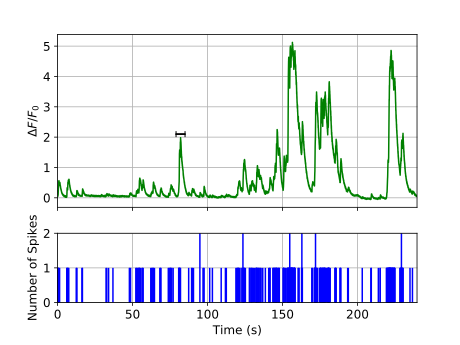
\includegraphics[width=\textwidth]{figures/spike_finder_example_8.png}
    \caption{}
  \end{subfigure}
  \begin{subfigure}{0.5\textwidth}
    \centering
    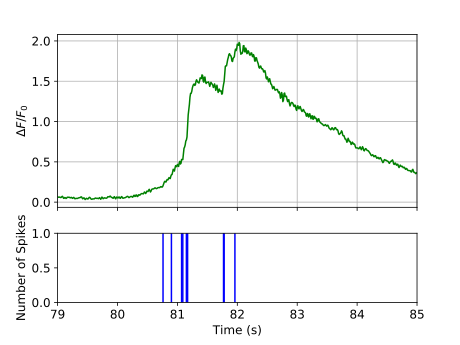
\includegraphics[width=\textwidth]{figures/spike_finder_example_8_zoomed.png}
    \caption{}
  \end{subfigure}
  \caption{(a) Plot of a spike train and the corresponding GCaMP6s fluorescence trace. Data courtesy of spikefinder.codeneuro.org (b) The same image as (a) but zoomed into the period from 79s to 85s. This period is marked on figure (a) by the horizontal black line with stars at each end. A group of six action potentials around the 81s point followed by a group of three action potentials just before the 82s point are shown. The decay of the fluorescence trace is much slower than the dynamics of an action potential.}
  \label{fig:spike_finder_example}
\end{figure}

\section{Results}

\subsection{The model}

\begin{figure}[p]
  \includegraphics[width=\textwidth]{figures/trace_comparison.png}
  \caption{(LHS) Observed fluorescence traces from the Spikefinder dataset with their associated spike trains. (RHS) Fluorescence traces created by the model given the same spike trains. Traces were created after the model was optimised for each florescence trace.}
  \label{fig:observed_modelled_examples}
\end{figure}

\begin{figure}
  \begin{subfigure}{0.5\textwidth}
    \includegraphics[width=\textwidth]{figures/concentration_dynamics.png}
    \caption{}
    \label{fig:contrentration_dynamics}
  \end{subfigure}
  \begin{subfigure}{0.5\textwidth}
    \includegraphics[width=\textwidth]{figures/concentration_dynamics_18_zoomed_BCa_star.png}
    \caption{}
  \end{subfigure}
  \begin{subfigure}{0.5\textwidth}
    \includegraphics[width=\textwidth]{figures/concentration_dynamics_18_zoomed_BCa.png}
    \caption{}
  \end{subfigure}
  \begin{subfigure}{0.5\textwidth}
    \includegraphics[width=\textwidth]{figures/concentration_dynamics_18_zoomed_ImCa.png}
    \caption{}
  \end{subfigure}
  \begin{subfigure}{0.5\textwidth}
    \includegraphics[width=\textwidth]{figures/concentration_dynamics_18_zoomed_ECa.png}
    \caption{}
  \end{subfigure}
  \begin{subfigure}{0.5\textwidth}
    \includegraphics[width=\textwidth]{figures/concentration_dynamics_18_zoomed_Ca.png}
    \caption{}
  \end{subfigure}
  \caption{\textbf{Calcium Buffering Dynamics } (a) The proportions of bound and free calcium concentrations within a cell, with the associated spike train. (b)-(f) The dynamics of the concentration of (b) excited indicator bound calcium, (c) indicator bound calcium, (d) immobile endogeneous buffer bound calcium, (e) mobile endogeneous buffer bound calcium, and (f) free calcium in response to an action potential at 23.17s.}
  \label{fig:concentrations}
\end{figure}

\subsection{Spike Inference}

\begin{figure}
  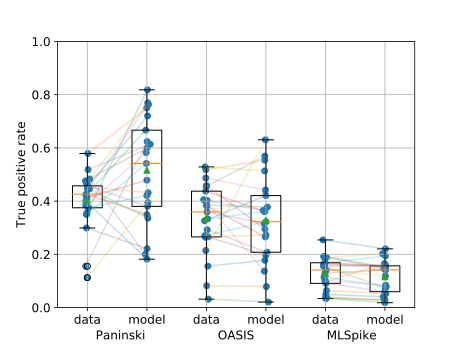
\includegraphics[width=\textwidth]{figures/three_algo_comparison_tp_paper.png}
  \caption{Box plots showing the distribution of the true positive rates achieved by three spike inference algorithms when applied to observed spike trains, and modelled spike trains. Data points overlaid as blue circles. The performance is similar from real and simulated data for each of the algorithms.}
  \label{fig:three_algo_comparison}
\end{figure}

\subsection{Perturbation analysis}

\subsubsection{Perturbing indicator concentration}

\begin{figure}
  \begin{subfigure}{\textwidth}
	   \includegraphics[width=\linewidth]{figures/indicator_perturbed_fluorescence_18_paper.png}
     \caption{}
  \end{subfigure}
  \begin{subfigure}{0.5\textwidth}
	   \includegraphics[width=\linewidth]{figures/indicator_perturbed_snr.png}
     \caption{}
  \end{subfigure}
  \begin{subfigure}{0.5\textwidth}
	   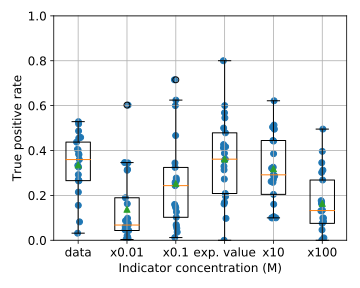
\includegraphics[width=\linewidth]{figures/indictor_perturbed_oasis_first_paper.png}
     \caption{}
  \end{subfigure}
  \caption{(a) An example trace for each of the five perturbed values for the concentration of fluorescent calcium indicator. The top two traces are produced by the lower perturbed values, the middle trace is produced by the experimental value, and the lowest two traces are produced when using the higher perturbed values. (b) The signal-to-noise ratio of the modelled fluorescence traces using each of the four perturbed values, and the experimental value. Extreme perturbations of the concentration either above or below the experimental level lowered the SNR. (c) The true-positive rates of the deconvolution algorithm's predictions when inferring from the observed data, and inferring from modelled traces using the perturbed and experimental values. We found that the algorithms performs equally badly on the two most extreme values, and performs equally well on the experimental value, and the next higher perturbed value.}
  \label{fig:indicator_perturbed}
\end{figure}

\subsubsection{Perturbing immobile endogeneous buffer concentration}

\begin{figure}
  \begin{subfigure}{\textwidth}
	   \includegraphics[width=\linewidth]{figures/immobile_perturbed_fluorescence_18_paper.png}
     \caption{}
  \end{subfigure}
  \begin{subfigure}{0.5\textwidth}
	   \includegraphics[width=\linewidth]{figures/immobile_perturbed_snr.png}
     \caption{}
  \end{subfigure}
  \begin{subfigure}{0.5\textwidth}
	   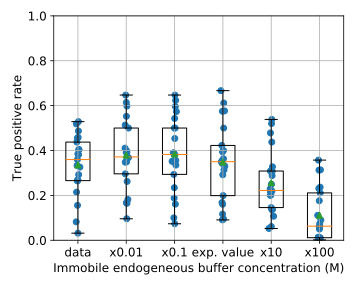
\includegraphics[width=\linewidth]{figures/immobile_perturbed_oasis_first_paper.png}
     \caption{}
  \end{subfigure}
  \caption{(a) An example trace for each of the five perturbed values for the concentration of immobile endogeneous buffer.	(b) The signal-to-noise ratio of the modelled fluorescence traces using each of the four perturbed values, and the experimental value. The lower values for the immobile buffer produce the same SNR as the experimental value. But the higher perturbed values produce fluorescence traces with a lower SNR.	(c) The true-positive rates of the deconvolution algorithm's predictions when inferring from the observed data, and inferring from modelled traces using the perturbed and experimental values.}
  \label{fig:endogeneous_perturbed}
\end{figure}

\subsubsection{Perturbing indicator binding and unbinding rates}

\begin{figure}
  \begin{subfigure}{\textwidth}
	   \includegraphics[width=\linewidth]{figures/b_i_f_i_perturbed_fluorescence_18_paper.png}
     \caption{}
  \end{subfigure}
  \begin{subfigure}{0.5\textwidth}
	   \includegraphics[width=\linewidth]{figures/b_i_f_i_perturbed_snr.png}
     \caption{}
  \end{subfigure}
  \begin{subfigure}{0.5\textwidth}
	   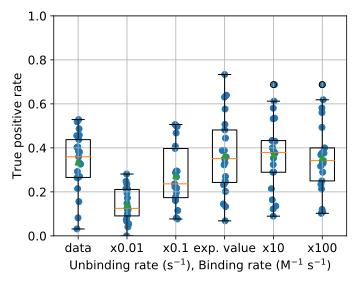
\includegraphics[width=\linewidth]{figures/b_i_f_i_perturbed_oasis_tp_paper.png}
     \caption{}
  \end{subfigure}
  \caption{(a) An example trace for each of the five pairs of values used for the binding and unbinding rates of the fluorescent calcium indicator. (b) The signal-to-noise ratio of the modelled fluorescence traces using each of the four perturbed values, and the experimental value. The SNRs for the two pairs with values lower than the experimental value are lower than the experimental pair or the higher value pairs. (c) The true-positive rates of the deconvolution algorithm's predictions when inferring from the observed data, and inferring from modelled traces using the perturbed and experimental values.}
  \label{fig:rates_perturbed}
\end{figure}

\subsection{Varying spike rate for different cell types}

\begin{figure}
  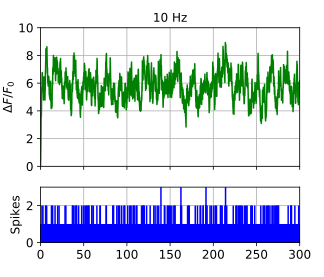
\includegraphics[width=0.329\linewidth]{figures/freq_compare_images_10_Hz_1_1.png}
  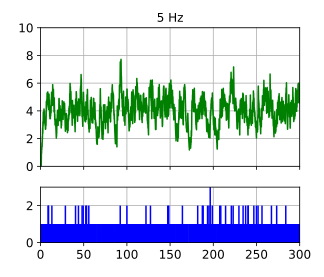
\includegraphics[width=0.329\linewidth]{figures/freq_compare_images_5_Hz_1_2.png}
  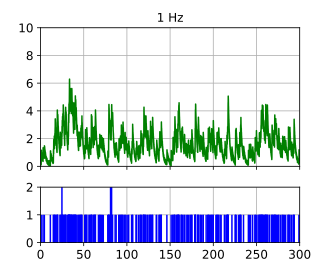
\includegraphics[width=0.329\linewidth]{figures/freq_compare_images_1_Hz_1_3.png}
  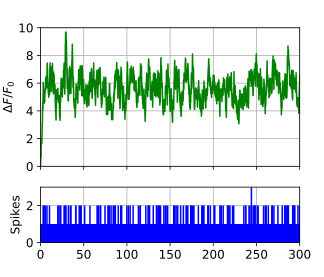
\includegraphics[width=0.329\linewidth]{figures/freq_compare_images_10_Hz_2_4.png}
  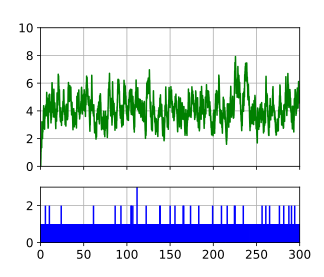
\includegraphics[width=0.329\linewidth]{figures/freq_compare_images_5_Hz_2_5.png}
  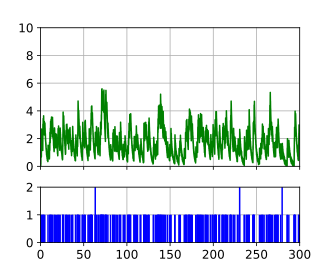
\includegraphics[width=0.329\linewidth]{figures/freq_compare_images_1_Hz_2_6.png}
  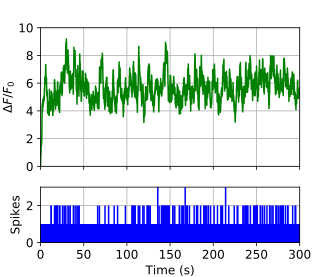
\includegraphics[width=0.329\linewidth]{figures/freq_compare_images_10_Hz_3_7.png}
  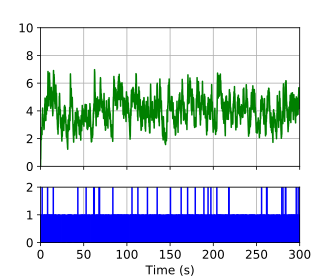
\includegraphics[width=0.329\linewidth]{figures/freq_compare_images_5_Hz_3_8.png}
  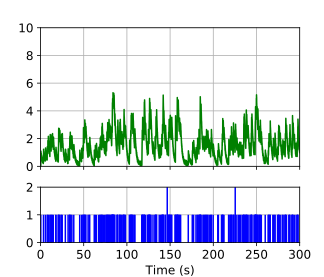
\includegraphics[width=0.329\linewidth]{figures/freq_compare_images_1_Hz_3_9.png}
  \caption{\textbf{Simulating fluorescence traces at different firing rates } Three example modelled traces created using simulated spike trains with a mean firing rate of 10 Hz (left column), 5 Hz (middle column), and 1 Hz (right column). Note the difference in amplitude with different mean firing rates.}
  \label{}
\end{figure}

\begin{figure}
  \includegraphics[width=0.5\linewidth]{figures/simulated_oasis_tp_paper.png}
  \includegraphics[width=0.5\linewidth]{figures/mean_fluorescence_comparison.png}
  \caption{(left) The spike inference true positive rate when applied to 30 traces created using simulated spike trains with mean firing rates of 1, 5, and 10 Hz. (right) The mean $\Delta F/F_0$ across those 30 traces for each frequency.}
  \label{}
\end{figure}




\end{document}

\chapter{Functional networks expand across anatomical boundaries as correlation time-scale increases}

\label{chap:eight_probe}

\subAbstract{Decades of research has established that correlated spiking plays a crucial role in representing sensory information. One drawback associated with the recent improvement in recording technology and consequent large datasets is the difficulty in analysing higher order correlations in large neuronal ensembles. One benefit of these datasets that has not yet been explored is the opportunity to compare correlations within anatomical regions to correlations across anatomical regions. In this work, we measured correlations between neurons residing in nine different brains regions in three awake and behaving mice. Using the these correlation measurements, we created weighted undirected graph networks and applied network science methods to detect functional communities in our neural ensembles. We compared these functional communities to their anatomical distribution. We repeated the analysis, using different timescales for our correlation measurements, and found that functional communities were more likely to be dominated by neurons from a single brain region at shorter timescales ($< 100$ms).}

\section{Introduction}
Decades of research has established that correlations play a crucial role in representing sensory information. For example, the onset of visual attention has been shown to have a greater affect on the correlations in the macaque V4 region than on the firing rates in that region  \parencite{cohen1}. Recent findings show that spontaneous behaviours explain correlations in parts of the brain not associated with motor control \parencite{stringer}, that satiety state appears to have a brain wide representation \parencite{allen}, and that subject exploratory and non-exploratory states are represented in the amygdala \parencite{grundemann}. So, behavioural states are likely represented across many regions of the brain, not just motor related areas. In order to understand the brain, we must understand the interactions between neurons and regions.

Because of limitations in recording technology almost all research has explored correlations between neurons within a given brain region, or within only two regions at most \parencite{wierzynski, patterson, girard}. Relatively little is known about correlations between neurons in many different brain regions. However, the recent development of `Neuropixels' probes  \parencite{jun} has allowed extracellular voltage measurements to be collected from multiple brain regions simultaneously routinely, and in much larger numbers than traditional methods. In this project we used a publicly-available Neuropixels dataset to analyse correlations between different brain regions  \parencite{stringer}.

A drawback associated with the improvement in recording technology is an increase in the difficulty in analysing these data. For example, analysing the $i$th order interactions of $N$ neurons generally requires estimation of $N^i$ parameters. A number that becomes astronomical for large $N$. New methods are required for analysing these new large datasets. We attempted to address this requirement in this piece of research by applying a cutting-edge network science community detection method to neural data.

Another unexplored area of research is the changes in cell interactions at different timescales. Studies have shown different timescales for fluctuations in spiking activity \parencite{murray}, and different time scales for event representation \parencite{baldassano} across different brain regions. Still most studies focus on quantifying interactions at a given timescale. But neurons may interact differently, or may interact with different neurons at different timescales. Here we explore correlated communities of neurons at different timescales.

In this work, we measured correlations between binned spike counts from neurons from nine different regions of the mouse brain. These measurements induced a weighted undirected graph or network where each neuron is represented by a node, and the strength of the connection between these nodes/neurons is the strength of the correlation between their spike counts. We then applied newly invented network methods \parencite{humphries} to this network to find any community structure, and place the neurons in these correlation based communities. Finally, we compared these functional communities to the anatomical membership of the neurons.

To investigate the functional communities and their relationship with anatomy at different time scales, we repeated these analyses using different length bin widths when binning spike times.

To find and analyse functional networks while controlling for the subject's behaviour, we conditioned the binned spike counts on data from a video of the subject's face, and repeated our analysis for spike count correlations (or noise correlations) and signal correlations.

\section{Results}

Note that in the following text, we refer to the correlation coefficient between two sequences of spike counts from two different cells as the \textit{total correlation}. We refer to the correlation between spike counts in response to a certain stimulus as the \textit{spike count correlation} aka \textit{noise correlation}, and we refer to the correlation between mean or expected responses to different stimuli as the \textit{signal correlation} \parencite{cohen2}.

The nine different brain regions from which we had data were the caudate putamen (CP), frontal motor cortex (FrMoCtx), hippocampus (HPF), lateral septum (LS), midbrain (MB), primary visual cortex (V1), superior colliculus (SC), somatomotor cortex (SomMoCtx), and thalamus (TH).

    \subsection{Average correlation size increases with increasing time bin width}
    First we inspected the affect of time bin width on total correlations. We know that using short time bins results in artificially small correlation measurements \parencite{cohen2}, so we expected to see an increase in correlation amplitude with increasing time bin width. That is exactly what we observed. Taking $50$ cells at random, we calculated the total correlation between every possible pair of these cells, using different time bin widths ranging from $0.005$s to $3$s. We found that the longer the time bin width, the greater the correlations (see figure \ref{fig:correlations_all_pairs}).

    \begin{figure}[h]
      \begin{subfigure}[h]{0.5\linewidth}
        \includegraphics[width=\linewidth]{figures/eight_probe/pairs_correlation.png}
        \caption{Correlation coefficient as a function of bin width.}
        \label{fig:pair_example_correlations}
      \end{subfigure}
      \begin{subfigure}[h]{0.5\linewidth}
        \includegraphics[width=\linewidth]{figures/eight_probe/pairs_raster.png}
        \caption{Raster plots for the four cells making up our example pairs.}
        \label{fig:pair_example_raster}
      \end{subfigure}
      \caption{(A) An example of the correlation coefficients between two different pairs of cells, one where both cells are in the same brain region (intra-regional pair), and one where both cells are in different brain regions (inter-regional pair). The correlation coefficients have been measured using different time bin widths, ranging from $5$ms to $3$s. Note the increasing amplitude of the correlations with increasing bin width. (B) A raster plot showing the spike times of each pair of cells.}
      \label{fig:pair_example}
    \end{figure}

    We also separated the positively correlated pairs from the negatively correlated pairs using the mean correlation of each pair across all bin widths (see section \ref{sec:corr_anti_corr}). We found that the positively correlated pairs become more positively correlated with increasing time bin width, and the negatively correlated pairs become more negatively correlated with increasing time bin width (see figures \ref{fig:correlations_pos_pairs} and \ref{fig:correlations_neg_pairs}).

    \begin{figure}[p]
        \begin{subfigure}[h]{0.5\linewidth}
            \includegraphics[width=\linewidth]{figures/eight_probe/Krebs_corr_all_pairs.png}
            \caption{All pairs, positive and negative.}
            \label{fig:correlations_all_pairs}
        \end{subfigure}
        \begin{subfigure}[h]{0.5\linewidth}
            \includegraphics[width=\linewidth]{figures/eight_probe/Krebs_corr_pos_pairs.png}
            \caption{All positively correlated pairs.}
            \label{fig:correlations_pos_pairs}
        \end{subfigure}
        \begin{subfigure}[h]{0.5\linewidth}
            \includegraphics[width=\linewidth]{figures/eight_probe/Krebs_corr_neg_pairs.png}
            \caption{All negatively correlated pairs.}
            \label{fig:correlations_neg_pairs}
        \end{subfigure}
        \begin{subfigure}[h]{0.5\linewidth}
            \includegraphics[width=\linewidth]{figures/eight_probe/Krebs_stats_by_bin_width.png}
            \caption{$\chi^2$ test statistics as goodness-of-fit.}
            \label{fig:chi_squared_fits}
        \end{subfigure}
        \caption{Mean correlation coefficients measured from pairs of $50$ randomly chosen neurons. (A) All possible pairs, (B) positively correlated pairs, and (C) negatively correlated pairs. (D) Mean and standard error of $\chi^2$ test statistics for Poisson and Gaussian distributions fitted to neuron spike counts.}
        \label{fig:correlations_vs_bin_widths}
    \end{figure}

    In figure \ref{fig:pair_example_correlations} we plot correlations from two example pairs, one pair from within a region, and one pair between regions. It can be seen that the correlation coefficient increases with bin width. The correlations can be observed by eye in the raster plot for these cells in figure \ref{fig:pair_example_raster}.

    When taking the mean across all pairs, the positively correlated pairs dominate in terms of both number of pairs, and amplitude of correlations. Therefore the mean across all pairs is positive.

    These results were observed in each of the three mouse subjects from which we had data.

    \subsection{Goodness-of-fit for Poisson and Gaussian distributions across increasing time bin widths}
    We wanted to investigate if the width of the time bin used to bin spike times into spike counts had an effect on the distribution of spike counts.  We used the $\chi^2$ statistic as a goodness-of-fit measure for Poisson and Gaussian (normal) distributions to the spike count of $100$ randomly chosen neurons for a number of bin widths ranging from $0.01$s to $4$s. For the $\chi^2$ statistic, the higher the value, the worse the fit.

    We expected a Poisson distribution to be a better fit for shorter time bin widths because spike counts must be non-negative, therefore any distribution of spike counts with mass distributed at or close to $0$ will be skewed. The distribution of spike counts is more likely to be distributed close to $0$ when the time bin widths used to bin spike times into spike counts are small relative to the amount of time it takes for a neuron to fire an action potential ($\sim 1$ms in the case of non-burst firing neurons).

    We expected a Gaussian distribution to be a better fit for longer time bin widths, because a Poisson distribution with a large rate is well approximated by a Gaussian distribution with mean and variance equal to the Poisson rate. Therefore, a Gaussian distribution would approximate the mean of a collection of large spike counts, and have more flexibility than a Poisson distribution to fit the variance.

    We found that that a Poisson distribution is the best fit for shorter time bins less than $0.7$s in length. Then a Gaussian distribution is a better fit for time bins greater than $0.7$s in length (see figure \ref{fig:chi_squared_fits}).

  \subsection{Differences between and inter- and intra- regional correlations decrease with increasing bin width}
  We investigated the differences in distribution between inter-regional correlations, i.e. correlations between neurons in different brain regions, and intra-regional correlations, i.e. correlations between neurons in the same brain region.

  Firstly, we investigated these quantities for all possible pairs of $\sim 500$ neurons taken from across all the $9$ brain regions from which we had data. We distributed these neurons as evenly as possible across all of the regions, so that cells from one region would not dominate our data. We observed that the mean intra-regional correlations were always higher than the mean inter-regional correlations for every value of time bin width used. We also observed that as the time bin width increased these mean correlations increased and the difference between the mean inter-regional and intra-regional correlations grew (see figure \ref{fig:all_pairs_inter_intra_corr} (Left)).

  Stringer et al. (2019) had a similar finding using the same data. They used only one value for the time bin width, $1.2$s. Using this time bin width to bin spike times and measure total correlations, they found that the mean `within-region' correlations were always greater than the `out-of-region' correlations  \parencite{stringer}. The figure from their paper showing this result can be seen in figure \ref{fig:all_pairs_inter_intra_corr} (Right).

  \begin{figure}[h]
    \includegraphics[width=0.5\linewidth]{figures/eight_probe/Krebs_inter_intra_regional_correlations.png}
    \includegraphics[width=0.5\linewidth]{figures/eight_probe/stringer_2019.png}
    \caption{(Left)The mean intra-region and inter-region correlations using all possible pairs of $\sim 500$ neurons, spread across $9$ different brain regions. (Right) Courtesy of Stringer et al. (2019), mean inter-regional (out-of-area) correlation coefficients vs  mean intra-regional (within-area) correlation coefficients for a bin width of 1.2s. Note that the intra-regional coefficients are higher in each case.}
    \label{fig:all_pairs_inter_intra_corr}
  \end{figure}

  Examples of the correlations of one intra-regional pair and one inter-regional pair can be seen in figure \ref{fig:pair_example}.

  Secondly, we separated those pairs into intra-regional and inter-regional groups. We noted that the mean intra-regional correlations (coloured dots in figures \ref{fig:short_bin_corr_comp} and \ref{fig:long_bin_corr_comp}) for a given region tended to be higher than the mean inter-regional correlations (black dots in figures \ref{fig:short_bin_corr_comp} and \ref{fig:long_bin_corr_comp}) involving cells from that region. However, in contrast with our previous result, we noted that the difference between the mean intra-regional correlations and most highly correlated inter-regional correlations reduced as we increased the time bin width (see figures \ref{fig:short_bin_corr_comp} and \ref{fig:long_bin_corr_comp}). This shows that the mean correlations showin in figure \ref{fig:all_pairs_inter_intra_corr} are not distributed evenly across all region pair combinations.

  \begin{figure}[p]
    \begin{subfigure}[h]{\linewidth}
      \centering
      \includegraphics[width=0.7\linewidth]{figures/eight_probe/Krebs_0p005_corr_comp.png}
      \caption{Mean inter-regional and intra-regional correlations using a time bin width of 5ms.}
      \label{fig:short_bin_corr_comp}
    \end{subfigure}
    \begin{subfigure}[h]{\linewidth}
      \centering
      \includegraphics[width=0.7\linewidth]{figures/eight_probe/Krebs_1p0_corr_comp.png}
      \caption{Mean inter-regional and intra-regional correlations using a time bin width of 1s.}
      \label{fig:long_bin_corr_comp}
    \end{subfigure}
    \caption{The mean intra-regional correlations (coloured dots) and mean inter-regional correlations (black dots) for a given region, indicated on the x-axis, for different time bin widths. Each black dot represents the mean inter-regional correlations between the region indicated on the x-axis and one other region. (A) shows these measurements when we used a time bin width of 5ms. (B) shows these measurements when we used a time bin width of 1s. Note that the difference between the mean inter-regional correlations and mean intra-regional correlations is smaller for 1s bins.}
    \label{fig:corr_comps}
  \end{figure}

  Finally, to see these regional mean correlations in a bit more detail, to examine the individual pair combinations in particular, we displayed these data in a matrix of mean correlations (see figure \ref{fig:corr_matrices}), showing the mean intra-regional correlations on the main diagonal, and the mean inter-regional correlations off diagonal. Comparing a version of this figure created using a short time bin width of $5$ms (figure \ref{fig:short_bin_corr_matrix}) and a version using a longer time bin width of $1$s (figure \ref{fig:long_bin_corr_matrix}) we observed that the mean intra-regional correlations are always relatively high in comparison to the mean inter-regional correlations, but the mean correlations in some inter-regional pairs are relatively much higher when using the longer time bin width.

  This could indicate information being processed quickly at a local or within-region level, and the local representations of this information spreading between regions at longer timescales.

  \begin{figure}[h]
    \begin{subfigure}[h]{0.5\linewidth}
      \centering
      \includegraphics[width=\linewidth]{figures/eight_probe/Krebs_0p005_corr_matrix.png}
      \caption{Time bin width 0.005s.}
      \label{fig:short_bin_corr_matrix}
    \end{subfigure}
    \begin{subfigure}[h]{0.5\linewidth}
      \centering
      \includegraphics[width=\linewidth]{figures/eight_probe/Krebs_1p0_corr_matrix.png}
      \caption{Time bin width 1s.}
      \label{fig:long_bin_corr_matrix}
    \end{subfigure}
    \caption{Mean inter-regional (main diagonal) and intra-regional (off diagonal) correlation coefficients. (A) Shows these measurements when spike times were binned using $5$ms time bins. (B) Shows the same, using $1$s time bins. Note that the matrices are ordered according to the main diagonal values, therefore the ordering is different in each subfigure.}
    \label{fig:corr_matrices}
  \end{figure}

  These results were consistent across the three mouse subjects. But, the relative magnitudes of the mean intra-regional and inter-regional correlations were not consistent. For example, the region with the highest mean intra-regional correlations when using $1$s bin widths for subject one is the superior colliculus (SC), but for subject two it is the midbrain (MB).

  \subsection{Connected and divided structure in correlation based networks reduces in dimension with increasing bin width}\label{sec:dims_result}
  We used the correlation measurements to create weighted undirected graphs/networks where each node represents a neuron, and the weight of each edge is the pairwise correlation between those neurons represented by the nodes at either end of that edge. We aimed to find communities of neurons within these networks, and compare the structure of these communities to the anatomical division of those neurons. The first step of this process involved applying the `spectral rejection' technique developed by Humphries et al (2019) \parencite{humphries}. This technique compares our data network to a chosen null network model, and finds any additional structure in the data network beyond that which is captured in the null network model (if there is any such structure).

  By comparing the eigenspectrum of the data network to the eigenspectrum of many samples from the null network model, this technique allows us to estimate the dimensionality of the additional structure in the data network, and gives us a basis for that vector space. It also divides the additional structure into connected structure, and $k$-partite (or divided) structure. For example, if our algorithm found two dimensions of additional connected structure, and one dimension of additional divided structure. We might expect to find three communities, that is groups more strongly connected within group that without, and we might expect to find bi-partite structure, that is two sets that are more strongly connected between groups than within groups.

  \begin{figure}[p]
    \begin{subfigure}[h]{0.5\linewidth}
      \centering
      \includegraphics[width=\linewidth]{figures/eight_probe/Krebs_rectified_total_structure_dims.png}
      \caption{Subject 1}
      \label{fig:Krebs_rectified_total_structure_dims}
    \end{subfigure}
    \begin{subfigure}[h]{0.5\linewidth}
      \centering
      \includegraphics[width=\linewidth]{figures/eight_probe/Waksman_rectified_total_structure_dims.png}
      \caption{Subject 2}
      \label{fig:Waksman_rectified_total_structure_dims}
    \end{subfigure}
    \begin{subfigure}[h]{0.5\linewidth}
      \centering
      \includegraphics[width=\linewidth]{figures/eight_probe/Robbins_rectified_total_structure_dims.png}
      \caption{Subject 3}
      \label{fig:Robbins_rectified_total_structure_dims}
    \end{subfigure}
    \caption{The number of dimensions in the $k$-partite and connected structure in the correlation based networks beyond the structure captured by a sparse weighted configuration null network model (see section \ref{sec:sparse_weighted_configuration_model}), shown for different time bin widths. Note that the $k$-partite structure disappears for time bin width greater than $200$ms for all three subjects. The dimension of the connected structure reduces with increasing bin width for $2$ of the $3$ subjects (top row).}
    \label{fig:structure_dims}
  \end{figure}

  The technique also finds which nodes contribute to this additional structure, and divides our data network into signal and noise networks. The details of spectral rejection and node rejection can be found in sections \ref{sec:spectral_rejection} and \ref{sec:node_rejection} respectively, and a full overview can be found in  \parencite{humphries}.

  We chose the sparse weighted configuration model (see section \ref{sec:sparse_weighted_configuration_model}) as our null network model. This model matches the sparsity and the total weight of the original network but distributes the weight at random across the sparse network.

  We applied the spectral rejection method to our networks based on total correlations using different values for the time bin width. We observed that for smaller time bin widths, our data networks had both $k$-partite structure, and community structure. As the width of the time bin increased, we found that the $k$-partite structure disappeared from our data networks, and the dimension of the community structure reduced in two of the three mice from which we had data (see figure \ref{fig:structure_dims}).

  \subsection{Detecting communities in correlation based networks}

  \begin{figure}[p]
    \begin{subfigure}[h]{0.5\linewidth}
      \includegraphics[width=\linewidth]{figures/eight_probe/Krebs_0p005_rectified_cons_cluster_map.png}
      \caption{5ms}
      \label{fig:consensus_cluster_5ms}
    \end{subfigure}
    \begin{subfigure}[h]{0.5\linewidth}
      \includegraphics[width=\linewidth]{figures/eight_probe/Krebs_1p0_rectified_cons_cluster_map.png}
      \caption{1s}
      \label{fig:consensus_cluster_1s}
    \end{subfigure}
    \begin{subfigure}[h]{0.5\linewidth}
      \includegraphics[width=\linewidth]{figures/eight_probe/Krebs_0p005_regional_cluster_map.png}
      \caption{5ms}
      \label{fig:regional_cluster_map_5ms}
    \end{subfigure}
    \begin{subfigure}[h]{0.5\linewidth}
      \includegraphics[width=\linewidth]{figures/eight_probe/Krebs_1p0_regional_cluster_map.png}
      \caption{1s}
      \label{fig:regional_cluster_map_1s}
    \end{subfigure}
    \caption{(A-B) Correlation matrices with detected communities indicated by white lines. Each off main diagonal entry in the matrix represents a pair of neurons. Those entries within a white square indicate that both of those neurons are in the same community as detected by our community detection procedure. Matrices shown are for $5$ms and $1$s time bin widths respectively. Main diagonal entries were set to $0$. (C-D) Matrices showing the anatomical distribution of pairs along with their community membership. Entries where both cells are in the same region are given a colour indicated by the colour bar. Entries where cells are in different regions are given the grey colour also indicated by the colour bar.}
    \label{fig:consensus_clusterings_with_regions}
  \end{figure}

  We applied the community detection procedure described in section \ref{sec:community_detection} to our signal networks for our various time bin widths. We detected a greater number of smaller communities at shorter time bin widths, and a smaller number of larger communities for longer time bin widths (see figure \ref{fig:consensus_clusterings_with_regions}). This was expected after the results found in section \ref{sec:dims_result}. We found more dimensions of additional structure at shorter time bin widths, therefore we found more communities at shorter time bin widths.

  We also noticed that at short time bin widths the communities detected tended to be dominated by cells from one region. Whereas communities existing in networks created using wider time bin widths tended to contain cells from many different brain regions. More on this in the next section.

% TODO: Need to expand the section in Methods on Community Detection.

  \subsection{Functional communities resemble anatomical division at short timescales}
  In order to quantify the similarity of the communities detected to the anatomical division of the cells. We treated both the anatomical division and the communities as clusterings of these cells. We then used measures for quantifying the difference or similarity between clusterings to quantify the difference or similarity between the detected communities and the anatomical division. Details of these measures can be found in section \ref{sec:clustering_comparison} or in  \parencite{vinh}.

  We used two different types of measures for clustering comparison; information based measures (see section \ref{sec:information_similarity_measures}) and pair counting based measures (see section \ref{sec:adjusted_rand_index}). We include one example of each in figure \ref{fig:distance_measures}.

  The variation of information is the information based measure included in figure \ref{fig:variation_of_information_rectified_total}. This measure forms a metric on the space of clusterings. The larger the value for the variation of information, the more different the clusterings.

  The adjusted Rand index is the pair counting based measure included in figure \ref{fig:adjusted_rand_index_rectified_total}. In contrast with the variation of information, the adjusted Rand index is a normalised similarity measure. The adjusted Rand index takes value 1 when the clusterings are identical, and takes value 0 when the clusterings are no more similar than chance.

  \begin{figure}[h]
    \begin{subfigure}[h]{0.5\linewidth}
      \includegraphics[width=\linewidth]{figures/eight_probe/variation_of_information_rectified_total.png}
      \caption{Variation of information}
      \label{fig:variation_of_information_rectified_total}
    \end{subfigure}
    \begin{subfigure}[h]{0.5\linewidth}
      \includegraphics[width=\linewidth]{figures/eight_probe/adjusted_rand_index_rectified_total.png}
      \caption{Adjusted Rand index}
      \label{fig:adjusted_rand_index_rectified_total}
    \end{subfigure}
    \caption{(A) The variation of information is a measure of distance between clusterings. The distance between the anatomical `clustering' and community detection `clustering' increases with increasing time bin width. (B) The adjusted Rand index is a normalised similarity measure between clusterings. The anatomical and community detection clusterings become less similar as the time bin width increases. }
    \label{fig:distance_measures}
  \end{figure}

  Both measures indicated that the detected communities and the anatomical division of the cells were more similar when we used shorter time bins widths (see figure \ref{fig:distance_measures}). This indicates that correlated behaviour in neuronal ensembles is more restricted to individual brain regions at short timescales ($<250$ms), and the correlated activity spreads out across brain regions over longer time scales.

  \subsection{Conditional correlations \& signal correlations}
  In light of the excellent research of Stringer et al (2019) showing that spontaneous behaviours can drive activity in neuronal ensembles across the visual cortex and midbrain \parencite{stringer}, we decided to control for the mouse's behaviour when performing our analyses. It is possible that our community detection process may be detecting communities across multiple brain regions at longer time scales due to aggregating neuronal activity driven by several spontaneous behaviours occurring during the time interval covered by a given time bin. A time bin of $1$s, for example, could contain a spike count where those spikes were driven by different spontaneous behaviours. We aimed to investigate this possibility by applying our community detection analysis to conditional correlation measures.

  \begin{figure}[h]
    \begin{subfigure}[h]{0.5\linewidth}
      \includegraphics[width=\linewidth]{figures/eight_probe/Krebs_cond_cov_comparison.png}
      \label{fig:Krebs_cond_cov_comparison}
    \end{subfigure}
    \begin{subfigure}[h]{0.5\linewidth}
      \includegraphics[width=\linewidth]{figures/eight_probe/Waksman_cond_cov_comparison.png}
      \label{fig:Waksman_cond_cov_comparison}
    \end{subfigure}
    \begin{subfigure}[h]{0.5\linewidth}
      \includegraphics[width=\linewidth]{figures/eight_probe/Robbins_cond_cov_comparison.png}
      \label{fig:Robbins_cond_cov_comparison}
    \end{subfigure}
    \caption{Comparing the components of the total covariance across different values for the time bin width. We observed a consistent increase in $E[\cov (X,Y|Z)]$ as the time bin width increased. But we saw different trends for $\cov (E[X|Z], E[Y|Z])$ for each mouse.}
    \label{fig:conditional_covariance_comparison}
  \end{figure}

  We used the top $500$ principal components of a video of the mouse's face as a measure of the mouse's behaviour (see section \ref{sec:video_recordings}). We modelled the spike counts as a linear combination of the principal components using linear regression with ElasticNet regularisation (see section \ref{sec:conditioning_on_behavioural_data}). Using this model, we quantified the expected spike count given the mouse's behaviour $E[X|Z_1, \dots ,Z_{500}]$.

  We used these expected values to measure $\cov (E[X|Z], E[Y|Z])$, and we used that value, the covariance $\cov (X,Y)$, and the \textit{law of total covariance} (see section \ref{sec:conditional_covariance}) to measure $E[\cov (X,Y|Z)]$. Here $X$ and $Y$ represent spike counts from individual cells, and $Z$ is shorthand for the $500$ principal components mentioned above. The two components of the covariance, $\cov (E[X|Z], E[Y|Z])$ and $E[\cov (X,Y|Z)]$, represent a `signal covariance' and expected value of a `spike count covariance' respectively, analagous to the signal correlation and spike count correlation \parencite{cohen2}.

  \begin{figure}[h]
    \begin{subfigure}[h]{0.5\linewidth}
      \includegraphics[width=\linewidth]{figures/eight_probe/Krebs_cond_corr_comparison.png}
      \label{fig:Krebs_cond_corr_comparison}
    \end{subfigure}
    \begin{subfigure}[h]{0.5\linewidth}
      \includegraphics[width=\linewidth]{figures/eight_probe/Waksman_cond_corr_comparison.png}
      \label{fig:Waksman_cond_corr_comparison}
    \end{subfigure}
    \begin{subfigure}[h]{0.5\linewidth}
      \includegraphics[width=\linewidth]{figures/eight_probe/Robbins_cond_corr_comparison.png}
      \label{fig:Robbins_cond_corr_comparison}
    \end{subfigure}
    \caption{Comparing the components of the total covariance across different values for the time bin width. We saw a consistent increase in $\rho_{X,Y|Z}$ as the time bin width increased in all three subjects. But we saw different trends in $\rho_{\text{signal}}$ for each of the subjects.}
    \label{fig:conditional_correlation_comparison}
  \end{figure}

  We examined the means of these components for different values of the time bin width (see figure \ref{fig:conditional_covariance_comparison}). We observed a consistent increase in $E[\cov (X,Y|Z)]$ as the time bin width increased. But we saw different trends for $\cov (E[X|Z], E[Y|Z])$ for each mouse.

  \begin{figure}[p]
    \begin{subfigure}[h]{0.5\linewidth}
      \includegraphics[width=\linewidth]{figures/eight_probe/Krebs_0p005_conditional_rectified_regional_cluster_map.png}
      \caption{$\rho_{X,Y|Z}$}
      \label{fig:short_time_conditional_rectified_regional_clusters}
    \end{subfigure}
    \begin{subfigure}[h]{0.5\linewidth}
      \includegraphics[width=\linewidth]{figures/eight_probe/Krebs_1p0_conditional_rectified_regional_cluster_map.png}
      \caption{$\rho_{X,Y|Z}$}
      \label{fig:long_time_conditional_rectified_regional_clusters}
    \end{subfigure}
    \begin{subfigure}[h]{0.5\linewidth}
      \includegraphics[width=\linewidth]{figures/eight_probe/Krebs_0p005_signal_rectified_regional_cluster_map.png}
      \caption{$\rho_{\text{signal}}$}
      \label{fig:short_time_signal_rectified_regional_clusters}
    \end{subfigure}
    \begin{subfigure}[h]{0.5\linewidth}
      \includegraphics[width=\linewidth]{figures/eight_probe/Krebs_1p0_signal_rectified_regional_cluster_map.png}
      \caption{$\rho_{\text{signal}}$}
      \label{fig:long_time_signal_rectified_regional_clusters}
    \end{subfigure}
    \caption{Matrices showing the regional membership of pairs by colour, and the communities in which those pairs lie. (A-B) Detected communities and regional membership matrix for network based on rectified spike count correlation $\rho_{X,Y|Z}$, using time bin widths of $0.005$s and $1$s respectively. (C-D) Detected communities and regional membership matrix for network based on rectified signal correlation $\rho_{\text{signal}}$, using time bin widths of $0.005$s and $1$s respectively.}
    \label{fig:rectified_signal_regional_clusters}
  \end{figure}

  Using $\cov (E[X|Z], E[Y|Z])$ we measured the signal correlation, $\rho_{\text{signal}}$, and using $E[\cov (X,Y|Z)]$ we measured the event conditional correlation, $\rho_{X,Y|Z}$ (see section \ref{sec:cond_corr} for more details). We saw a consistent increase in $\rho_{X,Y|Z}$ as the time bin width increased, this corresponds to the result for $E[\cov(X,Y|Z)]$. We observed different trends for $\rho_{\text{signal}}$ for each mouse, this corresponds to the result for $\cov(E[X|Z],E[Y|Z])$.

  We applied our network noise rejection and community detection process to networks based on the spike count correlations $\rho_{X,Y|Z}$ and the signal correlations $\rho_{\text{signal}}$. We noted that the community detection on $\rho_{X,Y|Z}$ behaved similarly to the community detection on the total correlation. We can see this  in figures \ref{fig:short_time_conditional_rectified_regional_clusters} and \ref{fig:long_time_conditional_rectified_regional_clusters}. At very short time bin widths, we detect more communities, and those communities often contain cells from one brain region only. At longer time bin widths, we detect fewer communities, and those communities tend to contain cells from multiple brain regions. When we examine the distance between (or similarity between) the anatomical division of the cells, and the detected communities we notice that the two clusterings are more similar at shorter time bin widths (see figure \ref{fig:conditional_clustering_distance_measures}).

  \begin{figure}[h]
    \begin{subfigure}[h]{0.5\linewidth}
      \includegraphics[width=\linewidth]{figures/eight_probe/variation_of_information_rectified_conditional.png}
      \caption{$\rho_{X,Y|Z}$ Variation of information.}
      \label{fig:variation_of_information_rectified_conditional}
    \end{subfigure}
    \begin{subfigure}[h]{0.5\linewidth}
      \includegraphics[width=\linewidth]{figures/eight_probe/adjusted_rand_index_rectified_conditional.png}
      \caption{$\rho_{X,Y|Z}$ Adjusted Rand Index.}
      \label{fig:adjusted_rand_index_rectified_conditional}
    \end{subfigure}
    \caption{Distance and similarity measures between the anatomical division of the neurons, and the communities detected in the network based on the spike count correlations $\rho_{X,Y|Z}$. (A) The variation of information is a `distance' measure between clusterings. The distance between the anatomical `clustering' and the community clustering increases as the time bin width increases. (B) The adjusted Rand index is a similarity measure between clusterings. The detected communities become less similar to the anatomical division of the cells as the time bin width increases.}
    \label{fig:conditional_clustering_distance_measures}
  \end{figure}

  \begin{figure}[h]
    \begin{subfigure}[h]{0.5\linewidth}
      \includegraphics[width=\linewidth]{figures/eight_probe/variation_of_information_rectified_signal.png}
      \caption{$\rho_{\text{signal}}$ Variation of information.}
      \label{fig:variation_of_information_rectified_signal}
    \end{subfigure}
    \begin{subfigure}[h]{0.5\linewidth}
      \includegraphics[width=\linewidth]{figures/eight_probe/adjusted_rand_index_rectified_signal.png}
      \caption{$\rho_{\text{signal}}$ Adjusted Rand Index.}
      \label{fig:adjusted_rand_index_rectified_signal}
    \end{subfigure}
    \caption{Distance and similarity measures between the anatomical division of the neurons, and the communities detected in the network based on the signal correlations $\rho_{\text{signal}}$. (A) The variation of information is a `distance' measure between clusterings. The distance between the anatomical `clustering' and the community clustering increases as the time bin width increases. (B) The adjusted Rand index is a similarity measure between clusterings. The detected communities become less similar to the anatomical division of the cells as the time bin width increases.}
    \label{fig:signal_clustering_distance_measures}
  \end{figure}

  When we applied the network noise rejection and community detection process to the networks based on the signal correlations $\rho_{\text{signal}}$ we found the number of communities we detected reduced with increasing time bin width. But the number of communities detected was less than that for the total correlations or the spike count correlations. The communities detected always tended to contain cells from multiple regions at both short and long timescales (see figures \ref{fig:short_time_signal_rectified_regional_clusters} and \ref{fig:long_time_signal_rectified_regional_clusters}). The communities detected bore very little relation to the anatomical division of the cells. The adjusted Rand index between the community clustering and the anatomical `clustering' is close to zero for every time bin width (see figure \ref{fig:adjusted_rand_index_rectified_signal}). This indicates that the similarity between the clusterings is close to chance. We did observe a slight downward trend in the variation of information with increasing bin width (see figure \ref{fig:variation_of_information_rectified_signal}), but this is more likely due to a decrease in the number of communities detected rather than any relationship with anatomy.

  We also observed that the network noise rejection process rejected some of the cells when applied to the network based on the signal correlations. This means that those cells did not contribute to the additional structure of the network beyond that captured by the sparse weighted configuration model. This is why the matrices in figures \ref{fig:short_time_signal_rectified_regional_clusters} and \ref{fig:long_time_signal_rectified_regional_clusters} are smaller than their analogues in figures \ref{fig:short_time_conditional_rectified_regional_clusters} and \ref{fig:long_time_conditional_rectified_regional_clusters}.

  % Figure 4: Conditional correlations
  % - Covariance matrices = conditional cov + signal cov
  % - Bar plot or similar comparing mean correlations for all three: total, conditional and signal.
  % - Corresponding plots for communities, one for conditional, one for signal, for both a short and long time bin
  % - VI measure vs time bins size for both types of correlation

  \subsection{Absolute correlations and negative rectified correlations}
  At the moment, the network noise rejection protocol can only be applied to weighted undirected graphs with non-negative weights. This meant that we had to rectify our correlated networks before applying the network noise rejection and community detection process. We wanted to investigate what would happen if instead of rectifying the correlations, we used the absolute value, or reversed the signs of the correlations and then rectified.

  \begin{figure}[p]
    \begin{subfigure}[h]{0.5\linewidth}
      \includegraphics[width=\linewidth]{figures/eight_probe/Krebs_0p005_absolute_cons_cluster_map.png}
      \caption{5ms}
      \label{fig:absolute_consensus_cluster_5ms}
    \end{subfigure}
    \begin{subfigure}[h]{0.5\linewidth}
      \includegraphics[width=\linewidth]{figures/eight_probe/Krebs_1p0_absolute_cons_cluster_map.png}
      \caption{1s}
      \label{fig:absolute_consensus_cluster_1s}
    \end{subfigure}
    \begin{subfigure}[h]{0.5\linewidth}
      \includegraphics[width=\linewidth]{figures/eight_probe/Krebs_0p005_regional_cluster_map_total_absolute.png}
      \caption{5ms}
      \label{fig:absolute_regional_cluster_map_5ms}
    \end{subfigure}
    \begin{subfigure}[h]{0.5\linewidth}
      \includegraphics[width=\linewidth]{figures/eight_probe/Krebs_1p0_regional_cluster_map_total_absolute.png}
      \caption{1s}
      \label{fig:absolute_regional_cluster_map_1s}
    \end{subfigure}
    \begin{subfigure}[h]{0.5\linewidth}
      \includegraphics[width=\linewidth]{figures/eight_probe/variation_of_information_absolute_total.png}
      \caption{Variation of information}
      \label{fig:variation_of_information_absolute_total}
    \end{subfigure}
    \begin{subfigure}[h]{0.5\linewidth}
      \includegraphics[width=\linewidth]{figures/eight_probe/adjusted_rand_index_absolute_total.png}
      \caption{Adjusted Rand index}
      \label{fig:adjusted_rand_index_absolute_total}
    \end{subfigure}
    \caption{(A-B) Absolute correlation matrices with detected communities indicated by white lines. These communities are based on the absolute value of the total correlation between each pair of cells. Those entries within a white square indicate that both of those neurons are in the same community. Matrices shown are for $5$ms and $1$s time bin widths respectively. Main diagonal entries were set to $0$. (C-D) Matrices showing the anatomical distribution of pairs along with their community membership. Regional membership is indicated by the colour bar. (E) Variation of information between the anatomical division of the cells, and the detected communities. (F) Adjusted Rand index between the anatomical division, and the detected communities.}
    \label{fig:absolute_consensus_clusterings_with_regions}
  \end{figure}

  \begin{figure}[p]
    \begin{subfigure}[h]{0.5\linewidth}
      \includegraphics[width=\linewidth]{figures/eight_probe/Krebs_0p005_negative_cons_cluster_map.png}
      \caption{5ms}
      \label{fig:negative_consensus_cluster_5ms}
    \end{subfigure}
    \begin{subfigure}[h]{0.5\linewidth}
      \includegraphics[width=\linewidth]{figures/eight_probe/Krebs_1p0_negative_cons_cluster_map.png}
      \caption{1s}
      \label{fig:negative_consensus_cluster_1s}
    \end{subfigure}
    \begin{subfigure}[h]{0.5\linewidth}
      \includegraphics[width=\linewidth]{figures/eight_probe/Krebs_0p005_regional_cluster_map_total_negative.png}
      \caption{5ms}
      \label{fig:negative_regional_cluster_map_5ms}
    \end{subfigure}
    \begin{subfigure}[h]{0.5\linewidth}
      \includegraphics[width=\linewidth]{figures/eight_probe/Krebs_1p0_regional_cluster_map_total_negative.png}
      \caption{1s}
      \label{fig:negative_regional_cluster_map_1s}
    \end{subfigure}
    \begin{subfigure}[h]{0.5\linewidth}
      \includegraphics[width=\linewidth]{figures/eight_probe/variation_of_information_negative_total.png}
      \caption{Variation of information}
      \label{fig:variation_of_information_negative_total}
    \end{subfigure}
    \begin{subfigure}[h]{0.5\linewidth}
      \includegraphics[width=\linewidth]{figures/eight_probe/adjusted_rand_index_negative_total.png}
      \caption{Adjusted Rand index}
      \label{fig:adjusted_rand_index_negative_total}
    \end{subfigure}
    \caption{(A-B) Sign reversed rectified correlation matrices with detected communities indicated by white lines. Those entries within a white square indicate that both of those neurons are in the same community. Matrices shown are for $5$ms and $1$s time bin widths respectively. Main diagonal entries were set to $0$. (C-D) Matrices showing the anatomical distribution of pairs along with their community membership. Regional membership is indicated by the colour bar. (E) Variation of information between the anatomical division of the cells, and the detected communities. (F) Adjusted Rand index between the anatomical division, and the detected communities.}
    \label{fig:negative_consensus_clusterings_with_regions}
  \end{figure}

  When we used the absolute value of the correlations, we found very similar results to those shown above for the rectified total correlations and the rectified spike count correlations. We detected more communities using shorter bin widths, and these communities were more similar to the brain's anatomy than those communities detected using a longer bin width (see figure \ref{fig:absolute_consensus_clusterings_with_regions}). The only exception being that we detected more communities. This could indicate that we detected both positively and negatively correlated communities, but we haven't done any further investigation so we cannot say for sure.

  When we used the sign reversed rectified correlated networks, we tended to find fewer communities. Each community contained cells from many different anatomical regions, at both long and short bin widths (see figures \ref{fig:negative_consensus_cluster_5ms}, \ref{fig:negative_consensus_cluster_1s}, \ref{fig:negative_regional_cluster_map_5ms}, \ref{fig:negative_regional_cluster_map_1s}). The communities bore little relation to the anatomical distribution of the cells, this can be seen in figure \ref{fig:adjusted_rand_index_negative_total}, the values close to zero indicate that the similarity between the two clusterings are around chance level. This indicates that there was not much structure in the negatively correlated networks beyond that captured by the sparse weighted configuration model.

\section{Discussion}
It is well established that the brain uses correlated behaviour in neuronal ensembles to represent the information taken in through sensation \parencite{cohen1, litwinkumar, decharms}. However, most studies that examine the nature of these correlations in-vivo, study an ensemble of cells from only one ot two brain regions \parencite{cohen2, wierzynski, patterson, girard}. Furthermore, recent results have shown that behaviour can drive correlated activity in multiple brain regions, including those not normally associated with motor control \parencite{stringer, grundemann, allen}. In this study, we utilised one of the newly recorded large datasets containing electrophysiological recordings from multiple brain regions simultaneously. We investigated correlated behaviour in these different brain regions and we investigated correlated behaviour between neurons in different regions, during spontaneous behaviour.

A number of studies have found that the timescale of correlated behaviour induced by a stimulus can be modulated by the stimulus structure and behavioural context. For example, the spike train correlations between cells in weakly electric fish are modulated by the spatial extent of the stimulus \parencite{litwinkumar}, and neurons in the marmoset primary auditory cortex modulate their spike timing (and therefore correlation) in response to stimulus features without modulating their firing rate  \parencite{decharms}. Furthermore, the width of the time bins over which spike counts are measured has been shown to have an effect on the magnitude of those correlations \parencite{cohen2}. Despite this, very little research has been done comparing correlation measures from the same dataset at different timescales. We investigated this by varying the time bin width used to bin spike times into spike counts from as short as $5$ms up to $3$s.

In order to further investigate the effect of these correlations at different timescales, we regarded our neuronal ensemble as a weighted undirected graph, where each neuron is represented by a node, and the weight on each edge is the correlation between the neurons connected by that edge. We then applied a novel clustering method from network science \parencite{humphries} to identify communities in these networks. Communities in a network graph refer to sets of nodes that are more strongly connected to each other than the nodes outside of their set. Another way to put this is to say that the nodes in a community are more strongly connected than \textit{expected}. What connection strength might be expected is defined by a null network model. We chose a null network model that matched the sparsity and total strength of our correlation based data networks. So, if two cells were in the same community, those cells were more correlated than would be expected given the correlation strength of their ensemble.

These networks, and the community detection process, were completely agnostic of the anatomical division of the cells in our ensemble. When we compared the detected communities with the anatomical division of the cells using distance and similarity measures for clusterings, we found that the detected communities were more similar to the anatomical division at shorter timescales. That is, when we used a wider time bin to count spikes, and computed pairwise correlations with these spike counts, the correlated communities tended to exist within anatomical regions at shorter timescales, and tended to span anatomical regions at longer timescales. This could reflect localised functional correlations at short time scales rippling outwards across brain regions at longer timescales. The brain may be processing some information quickly locally, and carrying out further, perhaps more detailed, representation over a longer timescale across many regions using the representations that were just built locally.

These changes in communities across timescales could also be driven by the anatomy of the individual cells. For example, it may simply take longer to transmit action potentials over longer distances, hence correlated activity over longer timescales will exist between anatomical regions, rather than within. However, the switch to almost exclusively multi-regional functional networks at $1$s bin widths, rather than a mixture of multi-region, and single-region suggests that the inter-regional correlations either overpower, or inhibit the local correlations. So there may be more at play than just timescales.

We acknowledged that the region spanning correlated communities that we detected at longer time scales could exist due to collating activity driven by distinct spontaneous activities. In order to account for this, we modelled the spike counts as a linear function of the top $500$ principal components of a video of the mouse's face filmed simultaneously with the electrophysiological readings. We applied our network noise rejection and community detection process to the weighted undirected networks formed by the spike count correlations (or noise correlations) and the signal correlations that we calculated using our model. For the spike count correlation networks, we found much the same results as for the total correlations as described above. For the signal correlations, the communities detected in these networks bore little relation to the anatomical division of the cells. Recent findings have shown that behavioural data accounts for correlations in many brain regions that would otherwise be dismissed as noise \parencite{stringer}, our finding to shows that these correlations are still governed by the timescale division between local communication and across-region communication.

There is a lot of room for further investigation based on this research. For a start, the data that we used here were collected from nine different regions in the mouse brain, but none of these regions were part of the somatosensory cortex. Given that a mouse experiences so much of its environment through its sense of smell, some data from this region would be interesting to investigate. On the same theme, the mice in the experiment from which the data were collected were headfixed and placed on a rotating ball, but were otherwise behaving spontaneously. Had these mice been exposed to a visual, aural, or olfactory stimulus, we could have examined the responses of the cells in the brain regions corresponding to vision, hearing, and olfaction, and compared these responses to the responses from the other brain regions. Furthermore, we could have investigated the interaction between the sets of responses.

Another space for further investigation is the community detection. The algorithm that we used here never detects overlapping communities. But functional communities could indeed have overlaps. Clustering methods that detect overlapping clusters do exist \parencite{baadel}. Applying one of those algorithms could yield some interesting results. Also, the community detection algorithm that we used here cannot process graphs with negative weights, this forced us to separate positive and negative correlations before applying our network noise rejection and community detections process, or use the absolute value of our correlations. A community detection algorithm that can work on weighted undirected graphs with negative weights could yield some interesting results here.

\section{Data}

    The data that we used in this project were collected by Nick Steinmetz and his lab members \parencite{stringer}.

    \subsection{Brain regions}
    Neuropixels probes were used to collect extracellular recordings  \parencite{jun} from three different mice. The mice were awake, headfixed, and engaging in spontaneous behaviour. The mice were of different sexes and different ages. One mouse was `wild-type', the others were mutants. Details as follows:
    \begin{enumerate}
        \item male, wild type, P73. % Robbins
        \item female, TetO-GCaMP6s, Camk2a-tTa, P113 % Waksman
        \item male, Ai32, Pvalb-Cre, P99 % Krebs
    \end{enumerate}

    Eight probes were used to collect readings from 2296, 2668, and 1462 cells respectively. Data were collected from nine brain regions in each mouse:
    \begin{itemize}
        \item Caudate Putamen (CP)
        \item Frontal Motor Cortex (Frmoctx)
        \item Hippocampal formation (Hpf)
        \item Lateral Septum (Ls)
        \item Midbrain (Mb)
        \item Superior Colliculus (Sc)
        \item Somatomotor cortex (Sommoctx)
        \item Thalamus (Th)
        \item Primary visual cortex (V1)
    \end{itemize}
    Readings were continuous and lasted for about 1 hour  \parencite{stringer}. Locations of each of the probes can be seen in figure \ref{fig:probe_locations}.

    \begin{figure}[h]
        \centering
        \includegraphics[width=5cm,height=3.75cm]{figures/eight_probe/probe_locations_stringer.png}
        \caption{\textbf{Probe Locations:} The locations of the probes in each of the three mouse brains \parencite{stringer}.}
        \label{fig:probe_locations}
    \end{figure}

    \subsection{Video recordings}\label{sec:video_recordings}
    Video recordings of the mouse's face were taken during the spontaneous behaviour. We had access to the top $500$ principle components and top $500$ eigenvectors of the processed videos. The frequency of recording was slightly less than $40$Hz. Each frame contained $327 \times 561$ pixels. These principal components were used as behavioural data. We controlled for these components when taking measurements conditioned on behaviour.

\section{Methods}
    \subsection{Binning data}
    We transformed the spike timing data into binned spike count data by dividing the experimental period into time bins and counting the spikes fired by each cell within the time period covered by each of those bins. The data were divided into time bins of various widths ranging from $0.01$s to $4$s.

    If the total length of the recording period was not an integer multiple of the time bin width, we cut off the remaining time at the end of the recording period. This period was at most $3.99$s. This is far less than the total recording time of around $1$ hour. So, this detail would not affect our results.

    \subsection{Correlation coefficients}
    We calculated Pearson's correlation coefficient for pairs of spike counts from pairs of neurons. For jointly distributed random variables $X$ and $Y$, Pearson's correlation coefficient is defined as:
    \begin{align}\label{eq:dist_pearsons_corr}
        \rho_{XY} =& \frac{\cov(X,Y)}{\sigma_X \sigma_Y} \\
                  =& \frac{E[(X - \mu_X)(Y - \mu_Y)]}{\sigma_X \sigma_Y}
    \end{align}
    where $E$ denotes the expected value, $\mu$ denotes the mean, and $\sigma$ denotes the standard deviation. The correlation coefficient is a normalised measure of the covariance. It can take values between $1$ (completely correlated) and $-1$ (completely anti-correlated). Two independent variables will have a correlation coefficient of $0$. But, having $0$ correlation does not imply independence.

    If we do not know the means and standard deviations required for equation \ref{eq:dist_pearsons_corr}, but we have samples from $X$ and $Y$, Pearson's sample correlation coefficient is defined as:
    \begin{align}
        r_{XY} = \frac{\sum_{i=1}^n (x_i - \bar{x})(y_i - \bar{y})}{\sqrt{\sum_{i=1}^n (x_i - \bar{x})^2}\sqrt{\sum_{i=1}^n (y_i - \bar{y})^2}}
    \end{align}
    where $\lbrace (x_i, y_i) \rbrace$ for $i \in \lbrace 1, \dots, n \rbrace$ are the paired samples from $X$ and $Y$, and $\bar{x} = \frac{1}{n}\sum_{i=1}^n x_i$, and $\bar{y} = \frac{1}{n}\sum_{i=1}^n y_i$ are the sample means.

    In practice we used the python function \texttt{scipy.stats.pearsonr} to calculate the correlation coefficients.

        \subsubsection{Total correlations, $r_{SC}$}\label{sec:spike_count_correlation}
        The total correlation ($r_{SC}$) of two cells is the correlation between the spike counts of those cells in response to a given stimulus condition.

        \subsubsection{Shuffled total correlations}\label{sec:shuffled_correlations}
        We measured the shuffled total correlations between two neurons by randomly permuting one of the neuron's spike counts and measuring the total correlations. These shuffled correlations were useful when measuring the effect of time bin width on correlations, and when deciding which correlations should be preserved when creating correlation networks (see section \ref{sec:sparsifying_data_networks}).

        \subsubsection{Separating Correlations \& Anti-correlations}\label{sec:corr_anti_corr}
        In order to compare the effect of bin width on measures of negative $r_{SC}$ (anti-correlation) and positive $r_{SC}$ separately, we had to separate correlated and anti-correlated pairs. To do this, we simply measured the mean $r_{SC}$, taking the mean across all the bin widths. If this quantity was positive or zero we regarded the pair as positively correlated. If this quantity was negative we regarded the pair as anti-correlated.

    \subsection{Conditioning on behavioural data}\label{sec:conditioning_on_behavioural_data}
    Our behavioural data consisted of the top $500$ principal components (PCs) of a processed video recording of the mouse's face (see section \ref{sec:video_recordings}). Denoting the spike count of a given cell by $X$, and the PCs by $Z_1,\dots,Z_{500}$, we wanted to model $X$ as a function of $Z_1,\dots,Z_{500}$ in order to estimate
    \begin{align}
      E[X|Z_1,\dots,Z_{500}] &= \int_{x \in X} x P(X=x | Z_1,\dots,Z_{500}) dx \\
        &= \int_{x \in X} x \frac{P(X=x, Z_1,\dots,Z_{500})}{P(Z_1,\dots,Z_{500})} dx
    \end{align}
    Given the $500$ components, a na\"{i}ve estimation of $P(Z_1,\dots,Z_{500})$ or $P(X, Z_1,\dots,Z_{500})$ by histogramming was impossible. Therefore we modelled $X$ as a linear combination of the PCs.

        \subsubsection{Linear regression}
        We modelled the spike count of a given cell, $X$, as a linear combination of the PCs of the video of the mouse's face, $\mathbf{Z} = Z_1,\dots,Z_{500}$. We tried three different types of regularization
        \begin{itemize}
            \item $L1$ or `Lasso'
            \item $L2$ or `Ridge regression'
            \item `Elastic net' regularisation (a linear combination of both $L1$ and $L2$ regularisation penalties)
        \end{itemize}
        The elastic net regularisation performed the best, so we stuck with that.

        \subsubsection{Elastic net regularisation}
        Suppose we wish to model $n$ observations of a random variable $X$, $\mathbf{x} = (x_1, \cdots, x_n)$ using $n$ instances of $m$ predictors $\mathbf{Z} = (Z_1, \cdots, Z_m)$. The na\"{i}ve elastic net criterion is
        \begin{align}\label{eq:elastic_net}
            L(\lambda_1, \lambda_2, \boldsymbol{\beta}) = | \mathbf{x} - \mathbf{Z} \boldsymbol{\beta} |^2 + \lambda_2 |\boldsymbol{\beta}|_2 + \lambda_1 |\boldsymbol{\beta}|_1
        \end{align}
        where
        \begin{align}
          |\boldsymbol{\beta}|_2 &= \sum_{j=1}^m \beta_j^2 \\
          |\boldsymbol{\beta}|_1 &= \sum_{j=1}^m |\beta_j|
        \end{align}
        The na\"{i}ve elastic net estimator $\hat{\boldsymbol{\beta}}$ is the minimiser of the system of equations \ref{eq:elastic_net}  \parencite{zou}
        \begin{align}
          \hat{\boldsymbol{\beta}} = \arg \min_{\boldsymbol{\beta}} L(\lambda_1, \lambda_2, \boldsymbol{\beta})
        \end{align}
        We implemented the model using the \texttt{ElasticNetCV} method of Python's \\ \texttt{sklearn.linear\_models} package.

        As well as using the PCs, we also tried fitting the models using the raw video data reconstructed from the PCs and eigenvectors. These models performed worse than those using the PCs. We expected this because each representation contains the same amount of information, but the raw video representation spreads this information across many more components. This requires more parameter fitting, but given the same information.

        \subsubsection{Conditional covariance}\label{sec:conditional_covariance}
        We calculated the expected value of the conditional covariance using the law of total covariance.
        \begin{align}\label{eq:law_of_total_covariance}
            \cov (X,Y) = E[ \cov(X,Y|Z)] + \cov(E[X|Z], E[Y|Z])
        \end{align}
        where these expected values are calculated with respect to the distribution of $Z$ as a random variable.

        The law of total covariance breaks the covariance into two components. The first component $E[\cov(X,Y|Z)]$ is the expected value, under the distribution of $Z$, of the conditional covariance $\cov(X,Y|Z)$. This covariance could be interpreted as the unnormalised version of what Cohen et al. (2011) call the spike count correlation \parencite{cohen2}, aka. the noise correlation. In particular, this is the covariance of the spike counts in response to repeated presentation of identical stimuli.

        The second component is analogous to what Cohn et al. (2011) call the \textit{signal correlation} \parencite{cohen2}. In particular, $\cov(E[X|Z], E[Y|Z])$ is the covariance between spike counts in response to different stimuli.

        Using our linear model, we calculated $E[X|Z_1,\dots, Z_{500}]$ for each cell $X$. Then we proceeded to calculate
        \begin{align}
            E[\cov(X,Y|Z_1,\dots, Z_{500})] = & \cov(X,Y) - \\
              & \cov(E[X|Z_1,\dots, Z_{500}], E[Y|Z_1,\dots, Z_{500}])
        \end{align}

        \subsubsection{Measures of conditional correlation}\label{sec:cond_corr}
        As a measure of expected correlation, we measured the `event conditional correlation'  \parencite{maugis}
        \begin{align}\label{eq:event_conditional_correlation}
            \rho_{XY|Z} = \frac{E[\cov(X,Y|Z)]}{\sqrt{E[\var(X|Z)]E[\var(Y|Z)]}}
        \end{align}
        Although this is not an actual correlation, it is an intuitive analogue to the correlation as a normalised version of the covariance.

        For comparison, we also measured the `signal correlation'
        \begin{align}\label{eq:signal_correlation}
            \rho_{\text{signal}} = \frac{\cov(E[X|Z], E[Y|Z])}{\sqrt{\var(E[X|Z])\var(E[Y|Z])}}
        \end{align}
        this is an actual correlation.

    \subsection{Information Theory}\label{sec:information_theory}
        \subsubsection{Entropy $H(X)$}
        The entropy of a random variable $X$, with outcomes $x_1, \dots, x_N$, and corresponding probabilities $p_1, \dots, p_N$ is defined as
        \begin{align}\label{entropy}
        H(X) = -\sum_{n=1}^N p_n \log _2 p_n
        \end{align}
        This quantity is also known as the information entropy or the `surprise'. It measures the amount of uncertainty in a random variable. For example, a variable with a probability of $1$ for one outcome, and $0$ for all other outcomes will have 0 bits entropy, because it contains no uncertainty. But a variable with a uniform distribution will have maximal entropy as it is the least predictable. This quantity is analogous to the entropy of a physical system  \parencite{shannon}. Note that any base may be used for the logarithm in equation \ref{entropy}, but using base $2$ means that the quantity will be measured in `bits'.

        The joint entropy of two jointly distributed random variables $X$ and $Y$, where $Y$ has outcomes $y_1, \dots, y_M$, is defined as
        \begin{align}\label{joint_entropy}
        H(X, Y) = -\sum_{n=1}^N \sum_{m=1}^M P(X=x_n, Y=y_m) \log _2 P(X=x_n, Y=y_m)
        \end{align}
        If $X$ and $Y$ are independent then $H(X,Y) = H(X) + H(Y)$. Otherwise $H(X,Y) < H(X) + H(Y)$. When $X$ and $Y$ and completely dependent $H(X,Y) = H(X) = H(Y)$.

        The conditional entropy of $Y$ conditioned on $X$ is defined as
        \begin{align}
        H(Y|X) = -\sum_{n=1}^N \sum_{m=1}^M P(X=x_n, Y=y_m) \log _2 \frac{P(X=x_n, Y=y_m)}{P(X=x_n)}
        \end{align}
        When $X$ and $Y$ are independent $H(Y|X) = H(Y)$. Intuitively, we learn nothing of $Y$ by knowing $X$, so $Y$ is equally uncertain whether we know $X$ or not. If $Y$ is totally dependent on $X$, then the fraction in the logarithm is $1$, which gives $H(Y|X) = 0$.

        These entropy measures are the basis of the mutual information measure.

        \subsubsection{Maximum entropy limit}\label{sec:entropy_limit}
        When spiking data is binned into spike counts there is an upper limit on the entropy of these data. The maximum entropy discrete distribution is the discrete uniform distribution. A random variable with this distribution will take values from some finite set with equal probabilities. Binned spike count data will take values between $0$ and some maximum observed spike count $n_{\max}$. A neuron with responses that maximises entropy will take these values with equal probability, i.e. if $i \in \lbrace 0, \dots, n_{\max} \rbrace$ then $P(X = i) = \frac{1}{n_{\max} + 1}$. The entropy of this neuron will be
        \begin{align*}
          H(X)  &= - \sum_{i=0}^{n_{\max}} P(X = i) \log _2 P(X=i) \\
                &= - \sum_{i=0}^{n_{\max}} \frac{1}{n_{\max} + 1} \log_2 \left( \frac{1}{n_{\max} + 1} \right) \\
                &= - \log_2 \left( \frac{1}{n_{\max} + 1} \right) \\
                &= \log_2 \left( n_{\max} + 1 \right)
        \end{align*}
        Therefore, the maximum entropy of the binned spike counts of a neuron is $\log _2 \left( n_{\max} + 1 \right)$. Of course, it would be very unusual for a neuron to fire in accordance with the discrete uniform distribution. Most measurements of entropy taken on binned spiking data will be much lower than the maximum. See figure \ref{fig:entropy_limit} to see the maximum entropy as a function of the maximum observed spike count.

        \begin{figure}[h]
          \centering
          \includegraphics[width=0.5\textwidth]{figures/eight_probe/entropy_limit.png}
          \caption{\textbf{Entropy Limit:} The upper limit on entropy of binned spike count data as a function of the maximum observed spike count. The orange line is the analytical maximum. The blue line is the entropy of samples with $N=1000$ data points taken from the discrete uniform distribution.}
          \label{fig:entropy_limit}
        \end{figure}

        \subsubsection{Mutual Information $I(X;Y)$}
        The mutual information can be defined mathematically in a number of ways, all of which are equivalent. These definitions illustrate the different ways of interpreting the mutual information.

        For two jointly distributed random variables $X$ and $Y$, the mutual information $I(X;Y)$ is defined as
        \begin{align}\label{eq:mutual_info_intuitive}
            I(X;Y)  =& H(Y) - H(Y|X) \\
                    =& H(X) - H(X|Y)
        \end{align}
        Equation \ref{eq:mutual_info_intuitive} fits with the following intuition: The mutual information between $X$ and $Y$ is the reduction in uncertainty about $X$ gained by knowing $Y$, or vice versa. We could also say the mutual information is the amount of information gained about $X$ by knowing $Y$, or vice versa.

        Another useful entropy based definition for the mutual information is
        \begin{align}\label{eq:mutual_info_useful}
            I(X;Y)  =& H(X) + H(Y) - H(X,Y)
        \end{align}
        This definition is useful because it does not require the calculation of conditional probabilities.

        The mutual information can also be defined in terms of marginal, joint, and conditional distributions. For example,
        \begin{align}\label{eq:mutual_info_log}
            I(X;Y)  =& -\sum_{n=1}^N \sum_{m=1}^M P(X=x_n, Y=y_m) \log _2 \frac{P(X=x_n, Y=y_m)}{P(X=x_n) P(Y=y_m)}
        \end{align}
        Notice that this can be rewritten as a Kullback–Leibler divergence.
        \begin{align}
            I(X;Y)  =& D_{KL}(P(X,Y)|| P(X)P(Y))
        \end{align}
        So, we can also think of the mutual information as a measure of the difference between the joint distribution of $X$ and $Y$, and the product of their marginal distributions. Since the product of the marginal distributions is the joint distribution for independent variables, we can think of the mutual information as a measure of the variables' dependence on one another.

        The minimum value that $I(X;Y)$ can take is $0$. This occurs when the random variables $X$ and $Y$ are independent. Then we have $H(X|Y) = H(X)$, and $H(Y|X) = H(Y)$, which according to equation \ref{eq:mutual_info_intuitive}, gives $I(X;Y) = 0$. We also have that $H(X,Y) = H(X) + H(Y)$ in this case, which according equation \ref{eq:mutual_info_useful}, gives $I(X;Y) = 0$. Finally, we also have $P(X,Y) = P(X)P(Y)$, which leaves us with $1$ in the argument for the logarithm in equation \ref{eq:mutual_info_log}, which again gives $I(X;Y) = 0$.

        The mutual information reaches its maximum value when one of the variables $X$ and $Y$ is completely determined by knowing the value of the other. In that case $I(X;Y) = \min \lbrace H(X), H(Y) \rbrace$.

        \subsubsection{Variation of Information $VI(X,Y)$}\label{sec:variation_of_information}
        The variation of information is another information theoretical quantity based on the mutual information. It is defined as
        \begin{align}\label{eq:variation_of_information}
            VI(X;Y) = H(X) + H(Y) - 2 I(X;Y)
        \end{align}
        We can rewrite this as the summation of two positive quantities
        \begin{align}
            VI(X;Y) = \left[ H(X) - I(X;Y) \right] + \left[ H(Y) - I(X;Y) \right]
        \end{align}
        In English, the variation of information is the summation of the uncertainty in the random variables $X$ and $Y$ excluding the uncertainty shared by those variables.

        This measure will become more relevant when we go on to talk about clusterings because $VI(X;Y)$ forms a metric on the space of clusterings.

        \subsubsection{Measuring entropies \& mutual information}
        In practice, we measured the mutual information between spike counts using Python and the python package \texttt{pyitlib}. We used the PT-bias correction technique to estimate the bias of our measurements when measuring the mutual information between the spike counts of two cells  \parencite{treves}.

        When measuring the mutual information between clusterings we used Python, but we used the \texttt{mutual\_info\_score}, \texttt{adjusted\_mutual\_info\_score}, and \\ \texttt{normalized\_mutual\_info\_score} functions from the \texttt{sklearn.metrics} part of the \texttt{sklearn} package.

    \subsection{Network analysis}
        \subsubsection{Correlation networks}
        In order to analyse functional networks created by the neurons in our ensemble, we measured the total correlation between each pair of neurons. These measurements induced an undirected weighted graph/network between the neurons. The weight of each connection was equal to the total correlation between each pair of neurons.

        We followed the same procedure for total correlations \ref{sec:spike_count_correlation}, spike count correlations, and signal correlations \ref{sec:cond_corr}.

        \subsubsection{Rectified correlations}
        At the time of writing, the community detection method outlined in  \parencite{humphries} could only be applied to networks with positively weighted connections. But many neuron pairs were negatively correlated. To apply the community detection method, we \textit{rectified} the network, by setting all the negative weights to zero.

        We also looked for structure in the network created by negative correlations by reversing the signs of the correlations, and rectifying these correlations before applying our network analysis.

        Finally, we used the absolute value of the correlations as the weights for the graph/network. By doing this, we hoped to identify both correlated and anti-correlated functional communities of neurons.

        \subsubsection{Sparsifying data networks}\label{sec:sparsifying_data_networks}
        When creating our correlation networks, we wanted to exclude any correlations that could be judged to exist `by chance'. To do this, we measured the $5$th and $95$th percentile of the shuffled correlations (see section \ref{sec:shuffled_correlations}) for the given mouse and time bin width. We then set all the data correlations between these two values to $0$. This excluded any `chance' correlations from our network, and created a sparser network. This allowed us to make use of the `sparse weighted configuration model' as described in section \ref{sec:sparse_weighted_configuration_model}.

        \subsubsection{Communities}
        Given some network represented by an adjacency matrix $\mathbf{A}$, a community within that network is defined as a collection of nodes where the number of connections within these nodes is higher than the expected number of connections between these nodes. In order to quantify the `expected' number of connections, we need a model of expected networks. This is analogous to a `null model' in traditional hypothesis testing. We test the hypothesis that our data network departs from the null network model to a statistically significant degree. For undirected unweighted networks, the canonical model of a null network is the configuration model  \parencite{fosdick}. Since we are working with weighted sparse networks, we used more suitable null models, described below.

        \subsubsection{Weighted configuration model}\label{sec:weight_configuration_model}
        The \textit{weighted configuration model} is a canonical null network model for weighted networks. Given some data network, the weighted configuration model null network will preserve the degree sequence and weight sequence of each node in the data network. But the edges will be distributed randomly  \parencite{fosdick}. Any structure in the data network beyond its degree sequence and weight sequence will not be captured in the weighted configuration model. So, this model can be used in testing the hypothesis that this extra structure exists.

        \subsubsection{Sparse weighted configuration model}\label{sec:sparse_weighted_configuration_model}
        The \textit{sparse weighted configuration model} is another null network model. Similar in nature to the weighted configuration model (see section \ref{sec:weight_configuration_model}), but the sparsity of the data network is preserved in the null network. This is achieved by sampling from a probability distribution for the creation or non-creation of each possible connection, then distributing the weight of the data network randomly in this sparse network  \parencite{humphries}. This is the null network that we used when searching for additional structure in our data networks.

        \subsubsection{Spectral rejection}\label{sec:spectral_rejection}
        We made use of the spectral rejection algorithm as outlined in  \parencite{humphries}. The spectral rejection algorithm is a method for finding structure in a network not captured by a supposed null model, if such structure exists.

        To describe the method, we denote our data network matrix $\mathbf{W}$, we denote the expected network of our null network model as $\left\langle \mathbf{P} \right\rangle$. Then the departure of our data network from the null network can be described by the matrix
        \begin{align}
          \mathbf{B} = \mathbf{W} - \left\langle \mathbf{P} \right\rangle
        \end{align}
        a common choice for $\left\langle \mathbf{P} \right\rangle$ in community detection is the `configuration model'  \parencite{fosdick, humphries2}. The matrix $\mathbf{B}$ is often called the configuration matrix, in this context we will use the term `deviation matrix' as it captures the deviation of $\mathbf{W}$ from the null model.

        To test for structure in the network represented by $\mathbf{W}$, we examine the eigenspectrum of $\mathbf{B}$ and compare it to the eigenspectrum of our null model. Firstly, note that since our data model doesn't allow self loops, and is not directed, the matrix representing the network will be symmetric and positive semi-definite, and will therefore be invertible with real eigenvalues. We selected a null model with the same characteristics.

        To find the eigenspectrum of the null model, we generated $N$ samples from our null model $P_1, \dots, P_N$, and we measured their deviation matrices $B_1, \dots, B_N$. We then calculated the eigenspectrum of each of those samples. We calculated the upper bound of the null model eigenspectrum by taking the mean of the largest eigenvalues of $B_1, \dots, B_N$. We calculated a lower bound on the null model eigenspectrum by taking the mean of the smallest eigenvalues of $B_1, \dots, B_N$.

        We then calculated the eigenspectrum of $\mathbf{B}$, our data network deviation matrix. If any of those eigenvalues lay outside of the upper or lower bounds of the null model eigenspectrum, this is evidence of additional structure not captured by the null model. If we chose the sparse weighted configuration model (see section \ref{sec:sparse_weighted_configuration_model}) as our null network model, then eigenvalues lying below the lower bound indicate $k$-partite structure in the network. For example, if one eigenvalue lay below the lower bound, this would indicate some bipartite structure in the data network. If any eigenvalues lay above the upper bound of the null model eigenspectrum, this is evidence of community structure in the data network. For example, one eigenvalue of $\mathbf{B}$ lying above the upper bound of the null model eigenspectrum indicates the presence of two communities in the network  \parencite{humphries2}.

        \subsubsection{Node rejection}\label{sec:node_rejection}
        If there are $d$ data eigenvalues lying outside of the null network eigenspectrum, the $d$ eigenvectors corresponding to these eigenvalues will form a vector space. If we project the nodes of our network into this vector space, by projecting either rows or columns of the data matrix, we can see how strongly each node contributes to the vector space. Nodes that contribute strongly to the additional structure will project far away from the origin, nodes that do not contribute to the additional structure will project close to the origin. We want to use this information to discard those nodes that do not contribute.

        We can test whether a node projects \textit{far} away from the origin or \textit{close} to the origin using the eigenvalues and eigenvectors of $B_1, \dots, B_N$. The $j$th eigenvector and eigenvalue of $B_i$ gives a value for a null network's projection into the $j$th dimension of the additional structure vector space. The matrices $B_1, \dots, B_N$ give $N$ projections into that dimension. These projections are a distribution of the null networks' projections. If the data node's projection exceeds that of the null network projections this node is judged to project \textit{far} from the origin, and therefore contribute to the additional structure. Otherwise, the node is judged to project \textit{close} to the origin, and is therefore rejected  \parencite{humphries}.

        \subsubsection{Community detection}\label{sec:community_detection}
        Another application for this $d$ dimensional space is community detection. We first project all of the nodes into this $d$-dimensional space, then perform the clustering in this space. The clustering and community detection procedure is described in  \parencite{humphries2}.

        In practice, the procedure is carried out $n$ times (we chose $n=100$ times), this returns $n$ clusterings. We resolve these $n$ clusterings to one final clustering using \textit{consensus clustering}. We used the consensus clustering method that uses an explicit null model for the consensus matrix, as outlined in  \parencite{humphries}.

    \subsection{Clustering Comparison}\label{sec:clustering_comparison}
    A clustering $\mathcal{C}$ is a partition of a set $D$ into sets $C_1, C_2, \dots, C_K$, called clusters, that satisfy the following for all $k,l \in \lbrace 1,\dots,K \rbrace$:
    \begin{align}
        C_k \cap C_l &= \emptyset \\
        \bigcup_{k=1}^K C_k &= D
    \end{align}
    If we consider two clusterings, $\mathcal{C}$ with clusters $C_1, C_2, \dots, C_K$ and $\mathcal{C}^{\prime}$ with clusters \\ $C_1^{\prime}, C_2^{\prime}, \dots, C_K^{\prime}$. There are a number of measurements we can use to compare $\mathcal{C}$ and $\mathcal{C}^{\prime}$. In the following, the number of elements in $D$ is denoted by $n$, and the number of elements in cluster $C_k$ is $n_k$.

      \subsubsection{Adjusted Rand Index}\label{sec:adjusted_rand_index}
      The \textit{adjusted Rand Index} is a normalised similarity measure for clusterings based on pair counting.

      If we consider the clusterings $\mathcal{C}$ and $\mathcal{C}^{\prime}$, and denote
      \begin{itemize}
        \item the number of pairs in the same cluster in $\mathcal{C}$ and $\mathcal{C}^{\prime}$ by $N_{11}$
        \item the number of pairs in different clusters in $\mathcal{C}$ and $\mathcal{C}^{\prime}$ by $N_{00}$
        \item the number of pairs in the same cluster in $\mathcal{C}$ and different clusters in $\mathcal{C}^{\prime}$ by $N_{10}$
        \item the number of pairs in different clusters in $\mathcal{C}$ and the same cluster in $\mathcal{C}^{\prime}$ by $N_{01}$
      \end{itemize}
      then the \textit{Rand Index} is defined as
      \begin{align}
          RI = \frac{N_{11} + N_{00}}{N_{11} + N_{00} + N_{10} + N_{01}} = \frac{N_{11} + N_{00}}{\binom{n}{2}}
      \end{align}
      The Rand Index is $1$ when the clusterings are identical, and $0$ when the clusterings are completely different.

      The \textit{adjusted Rand Index} intends on correcting the Rand Index for chance matching pairs. This is defined as
      \begin{align}
          ARI = \frac{2\left( N_{00}N_{11} - N_{01}N_{10} \right)}{\left( N_{00} + N_{01} \right)\left( N_{01} + N_{11} \right) + \left( N_{00} + N_{10} \right)\left( N_{10} + N_{11} \right)}
      \end{align}
      The adjusted Rand Index is $1$ when the clusterings are identical, and $0$ when the Rand Index is equal to its expected value.

      \subsubsection{Clusterings as random variables}
      If we take any random element of $D$, the probability that this element is in cluster $C_k$ of clustering $\mathcal{C}$ is
      \begin{align}
          P(K=k) = \frac{n_k}{n}
      \end{align}
      this defines a probability distribution, which makes the clustering a random variable. Any clustering can be considered as a random variable this way.

      This means that we can measure any of the information theoretic quantities defined in section \ref{sec:information_theory} with respect to clusterings. For example, the entropy of a clustering is
      \begin{align}
          H(\mathcal{C}) = - \sum_{k=1}^K \frac{n_k}{n} \log \frac{n_k}{n}
      \end{align}
      If we have two clusterings, the joint probability distribution of these clusterings is defined as
      \begin{align}
          P(K=k,K^{\prime}=k^{\prime}) = \frac{|C_k \cap C^{\prime}_{k^\prime}|}{n}
      \end{align}
      The joint distribution allows us to define the mutual information between two clusterings, $I(\mathcal{C};\mathcal{C}^{\prime})$  \parencite{meila}.

      \subsubsection{Information based similarity measures}\label{sec:information_similarity_measures}
      The mutual information between two clusterings is a similarity measure, with $I(\mathcal{C};\mathcal{C}^{\prime}) = 0$ if $\mathcal{C}$ and $\mathcal{C}^{\prime}$ are completely different, and $I(\mathcal{C};\mathcal{C}^{\prime}) = H(\mathcal{C}) = H(\mathcal{C}^{\prime})$ if $\mathcal{C}$ and $\mathcal{C}^{\prime}$ are identical. This can be normalised in a number of different ways to make more similarity measures  \parencite{vinh}
      \begin{align}
          NMI_{joint} &= \frac{I(\mathcal{C};\mathcal{C}^{\prime})}{H(\mathcal{C}, \mathcal{C}^{\prime})} \\
          NMI_{max} &= \frac{I(\mathcal{C};\mathcal{C}^{\prime})}{\max \lbrace H(\mathcal{C}), H(\mathcal{C}^{\prime}) \rbrace} \\
          NMI_{sum} &= \frac{2I(\mathcal{C};\mathcal{C}^{\prime})}{H(\mathcal{C}) + H(\mathcal{C}^{\prime}) } \\
          NMI_{sqrt} &= \frac{I(\mathcal{C};\mathcal{C}^{\prime})}{\sqrt{H(\mathcal{C}) H(\mathcal{C}^{\prime}) }} \\
          NMI_{min} &= \frac{I(\mathcal{C};\mathcal{C}^{\prime})}{\min \lbrace H(\mathcal{C}), H(\mathcal{C}^{\prime}) \rbrace}
      \end{align}
      We can control for chance similarities between the two clusterings by measuring the \textit{adjusted mutual information} between the clusterings. This is defined as
      \begin{align}
        AMI_{sum} = \frac{I(\mathcal{C};\mathcal{C}^{\prime}) - E \lbrace I(\mathcal{C};\mathcal{C}^{\prime}) \rbrace}{\frac{1}{2}\left[ H(\mathcal{C}) + H(\mathcal{C}^{\prime})\right] - E \lbrace I(\mathcal{C};\mathcal{C}^{\prime})  \rbrace}
      \end{align}
      The first term in the denominator, taking the average of the marginal entropies, can be replaced by taking the maximum, minimum, or the geometric mean  \parencite{vinh}.

      \subsubsection{Information based metrics}\label{sec:information_metrics}
      The variation of information between two clusterings $VI(\mathcal{C};\mathcal{C}^{\prime})$ (see section \ref{sec:variation_of_information}) is a metric on the space of clusterings  \parencite{meila}. That is,
      \begin{align}
          VI(\mathcal{C};\mathcal{C}^{\prime}) &\geq 0 \\
          VI(\mathcal{C};\mathcal{C}^{\prime}) &= 0 \iff \mathcal{C} = \mathcal{C}^{\prime} \\
          VI(\mathcal{C};\mathcal{C}^{\prime}) &= VI(\mathcal{C}^{\prime};\mathcal{C}) \\
          VI(\mathcal{C};\mathcal{C}^{\prime \prime}) &\leq VI(\mathcal{C};\mathcal{C}^{\prime}) + VI(\mathcal{C}^{\prime};\mathcal{C}^{\prime \prime})
      \end{align}

      Another metric is the \textit{information distance}  \parencite{vinh}
      \begin{align}
          D_{max} = \max \lbrace H(\mathcal{C}), H(\mathcal{C}^{\prime}) \rbrace - I(\mathcal{C};\mathcal{C}^{\prime})
      \end{align}

      Both of these can be normalised
      \begin{align}
          NVI(\mathcal{C};\mathcal{C}^{\prime}) & = 1 - \frac{I(\mathcal{C};\mathcal{C}^{\prime})}{H(\mathcal{C}, \mathcal{C}^{\prime})} \\
          d_{max} & = 1 - \frac{I(\mathcal{C};\mathcal{C}^{\prime})}{\max \lbrace H(\mathcal{C}), H(\mathcal{C}^{\prime}) \rbrace}
      \end{align}

      \subsubsection{Comparing detected communities and anatomical divisions}
      In order to quantify the difference or similarity between the communities detected in our correlation network and the anatomical classification of the cells in that network, we considered the communities and the anatomical regions as clusters in two different clusterings, $\mathcal{C}_{comm}$ and $\mathcal{C}_{anat}$, respectively. We then measured the similarity between the clusterings using the mutual information, the adjusted mutual information, and the normalised mutual information. We measured the difference between, or the distance between, the clusterings using the variation of information, the normalised variation of information, and the normalised information distance. We also measured the difference between the clusterings using the adjusted Rand Index, just to use a non-information based measure.

      We took all of these measures for communities detected using different time bin widths. This gave us an idea of the effect of time bin width on correlation networks in neural ensembles relative to anatomical regions within those ensembles.


\chapter{A simple two parameter distribution for modelling neuronal activity and capturing neuronal association}

\label{chap:comb}

\subAbstract{Recent developments in electrophysiological technology have lead to an increase in the size of electrophysiology datasets. Consequently, there is a requirement for new analysis techniques that can make use of these new datasets, while remaining easy to use in practice. In this work, we fit some one or two parameter probability distributions to spiking data collected from a mouse exposed to visual stimuli. We show that the Conway-Maxwell-binomial distribution is a suitable model for the number of active neurons in a neuronal ensemble at any given moment. This distribution fits these data better than binomial or beta-binomial distributions. It also captures the correlated activity in the primary visual cortex induced by stimulus onset more effectively than simply measuring the correlations, at short timescales ($<10$ms). We also replicate the finding of Churchland et al (2010) relating to stimulus onset quenching neural variability in cortical areas, and we show a correspondence between this quenching and changes in one of the parameters of the fitted Conway-Maxwell-binomial distributions.}

\section{Introduction}
Recent advances in electrophysiological technology, such as `Neuropixels' probes \parencite{jun} have allowed extracellular voltage measurements to be collected from larger numbers of cells than traditional methods, in multiple brain regions simultaneously, and routinely. These larger datasets require innovative methods to extract information from the data in a reasonable amount of time, `reasonable' being subjective in this case.

Theoretically, all the information at any given moment in an electrophysiological dataset with $n$ neurons could be captured by calculating the probability distribution for every possible spiking pattern. This would require defining a random variable with $2^n$ possible values, a task that quickly becomes impossible as $n$ increases. Attempts at approximating this random variable often involve measuring pairwise or higher order correlations  \parencite{schneidman, flach, ganmor}. But pairwise correlations may not be enough to characterise instantaneous neural activity \parencite{tkacik}. Furthermore, these kinds of models tend to ignore the temporal structure of neuronal data, in favour of smaller model size, and scalability.

Higher order correlations would be helpful here, but defining and quantifying these correlations can be tricky \parencite{staude}. If we use the interaction parameters arising from the exponential family model as measures of higher order correlations, measuring these correlations becomes computationally impractical quite quickly (the number of `three neuron correlations' to measure scales with $\binom{n}{3}$). In this work, we dispense with measuring correlations directly, and we attempt to characterise correlated behaviour using a parameter in statistical model.

In this work, we examined the ability of simple distributions to model the number of active (spiking) neurons in a neuronal ensemble at any given timepoint. We compared a little-known distribution named the Conway-Maxwell-binomial distribution to the binomial distribution and the beta-binomial distribution. The binomial distribution is a probability distribution over the number of successes is a sequence of independent and identical Bernoulli trials. The beta-binomial distribution is similar, but allows for a bit more flexibility while still being a model for heterogeneity. Similar to the binomial and beta-binomial, the Conway-Maxwell-binomial distribution is a probability distribution over the number of successes in a series of Bernoulli trials, but allows over- and under-dispersion relative to the binomial distribution. This distribution should therefore be a good candidate for our purposes. We found that Conway-Maxwell-binomial distribution was usually the best candidate of the three that we examined.

We also observed some interesting changes in the number of active neurons in the primary visual cortex and hippocampus at stimulus onset and some changes in this activity in the thalamus which were sustained for the full duration of the stimulus presentation. This let us know that there were some responses to model.

We found that fitting a Conway-Maxwell-binomial distribution was a better method of capturing association between neurons than measuring the spike count correlation for the short time bins that we used ($<10$ms).

Finally, we also wanted to investigate parallels between the parameters of the Conway-Maxwell-binomial distribution and quantities that have been established as relevant to sensory processing. So, we replicated the findings made by Churchland et al. (2010) relating to a reduction in neural variability at stimulus onset in the macaque cortical regions, but for data taken from the mouse primary visual cortex. We compared these findings to the values of the fitted Conway-Maxwell-binomial distribution parameters.

\section{Data}
We used data collected by Nick Steinmetz and his lab `CortexLab at UCL'  \parencite{steinmetz}. The data can be found online \footnote{\url{http://data.cortexlab.net/dualPhase3/}} and are free to use for research purposes.

Two `Phase3' Neuropixels  \parencite{jun} electrode arrays were inserted into the brain of an awake, head-fixed mouse for about an hour and a half. These electrode arrays recorded $384$ channels of neural data each at $30$kHz and  less than $7\mu$V RMS noise levels. The sites are densely spaced in a `continuous tetrode'-like arrangement, and a whole array records from a $3.8$mm span of the brain. One array recorded from visual cortex, hippocampus,  and thalamus, the other array recorded from motor cortex and striatum. The data were spike-sorted automatically by Kilosort and manually by Nick Steinmetz using Phy. In total 831 well-isolated individual neurons were identified.

  \subsection{Experimental protocol}\label{sec:experimental_protocal}
  The mouse was shown a visual stimulus on three monitors placed around the mouse at right angles to each other, covering about $\pm 135$ degrees azimuth and $\pm 35$ degrees elevation.

  The stimulus consisted of sine-wave modulated full-field drifting gratings of 16 drift directions ($0^{\circ}, 22.5^{\circ}, \dots, 337.5^{\circ}$) with $2$Hz temporal frequency and $0.08$ cycles/degree spatial frequency displayed for $2$ seconds plus a blank condition. Each of these $17$ conditions were presented $10$ times in a random order across $170$ different trials. There were therefore $160$ trials with a drifting-grating visual stimulus present, and $10$ trials with a blank stimulus.

\section{Methods}

    \subsection{Binning data}
    We converted the spike times for each cell into spike counts by putting the spike times into time bins of a given `width' (in milliseconds). We used time bins of $1$ms, $5$ms, and $10$ms. We used different time bin widths to assess the impact of choosing a bin width.


    \subsection{Number of \textit{active} neurons}\label{sec:num_active_neurons}
    To count the number of active neurons in each neuronal ensemble, we split the time interval for each trial into bins of a given width. We counted the number of spikes fired by each cell in each bin. If a cell fired \textit{at least} one spike in a given bin, we regarded that cell as active in that bin. We recorded the number of active cells in every bin, and for the purposes of further analysis, we recorded each cell's individual spike counts.

    It should be noted that when we used a bin width of $1$ms, the maximum number of spikes in any bin was $1$. For the wider time bins, some bins had spike counts greater than $1$. Consequently when using a bin width of $1$ms, the number of active neurons and the total spike count of a given bin were identical. But for wider bin widths, the total spike count was greater than the number of active neurons.

    So for the $1$ms bin width, the activity of a neuron and the number of spikes fired by that neuron in any bin can be modelled as a Bernoulli variable. But for wider time bins, only the activity can be modelled in this way.

    \subsection{Moving windows for measurements}

    When taking measurements (e.g. moving average over the number of active neurons) or fitting distributions (eg. the beta binomial distribution) we slid a window containing a certain number of bins across the data, and made our measurements at each window position. For example, when analysing $1$ms bin data, we used a window containing $100$ bins, and we slid the window across the time interval for each trial moving $10$ bins at a time. So that for $3060$ms of data, we made $296$ measurements.

    For the $5$ms bin width data, we used windows containing $40$ bins, and slid the window $2$ bins at a time when taking measurements.

    For the $10$ms bin width data, we used windows containing $40$ bins, and slid the window $1$ bin at a time when taking measurements (see table \ref{tab:bin_widths} for concise details).

    By continuing to use windows containing $40$ bins, we retained statistical power but sacrificed the number of measurements taken.

    \begin{table}
      \centering
      \begin{tabular}[h]{|c|c|c|c|}
        \hline
        \textbf{Bin width (ms)}   & \textbf{Window size (bins)}   & \textbf{Window size (ms)} & \textbf{Windows per trial}  \\ \hline
        $1$ms                     & $100$                         & $100$ms                   & $296$                       \\ \hline
        $5$ms                     & $40$                          & $200$ms                   & $286$                       \\ \hline
        $10$ms                    & $40$                          & $400$ms                   & $266$                       \\ \hline
      \end{tabular}
      \caption{Details of the different bin width and analysis window sizes used when binning spike times, and analysing those data.}
      \label{tab:bin_widths}
    \end{table}

    There was an interval between each trial with a grey image in place of the moving of the moving bar stimulus. This interval varied in time. But we included some of this interval when recording the data for each trial. We started recording the number of active neurons, and the number of spikes from each neuron from $530$ms before each trial until $1030$ms after each trial. This way, we could see the change in our measurements at the onset of a stimulus and the end of stimulus presentation.

    As mentioned in section \ref{sec:num_active_neurons}, we recorded the number of active neurons in each bin, and the spike count for each neuron in each bin. The actual measurements we took using these data in each window were as follows:
    \begin{description}
      \item[Moving average] The average number of active cells in each window.
      \item[Moving variance] The variance of the number of active cells in each window.
      \item[Average correlation] We measured the correlation between the spike counts of each pair of cells in the ensemble, and took the average of these measurements.
      \item[Binomial \textit{\textbf{p}}] We fitted a binomial distribution to the data in each window and recorded the fitted probability of success, $p$ in each case.
      \item[Beta-binomial $\boldsymbol{\alpha}$, $\boldsymbol{\beta}$] We fitted a beta-binomial distribution to the data in each window, and recorded the values of the fitted shape parameters, $\alpha$ and $\beta$, of each distribution.
      \item[Conway-Maxwell-binomial distribution \textit{\textbf{p}}, $\boldsymbol{\nu}$] We fitted a Conway-Maxwell-binomial distribution to the data in each window, and recorded the fitted values of $p$ and $\nu$ for each distribution.
      \item[Log-likelihoods] We also recorded the log-likelihood of each of the fitted distributions for each window.
    \end{description}

    \subsection{Fano factor}\label{sec:fano_factor}
    The \textit{Fano factor} of a random variable is defined as the ratio of the variable's variance to its mean.
    \begin{align}\label{eq:fano_factor}
      F = \frac{\sigma^2}{\mu}
    \end{align}
    We measured the Fano factor of the spike count of a given cell by measuring the mean and variance of the spike count across trials, and taking the ratio of those two quantities. When calculated in this way the Fano factor can be used as a measure of neural variability that controls for changes in the firing rate.  This is similar to the calculation used in \parencite{Churchland}.

    \subsection{Probability Distributions suitable for modelling ensemble activity}

    We present here three different probability distributions that could be suitable to model the number of active neurons in an ensemble. Each distribution has the set $\lbrace 0, \dots, n \rbrace$ as its support, where $n$ is the number of neurons in the ensemble. These are simple distributions with either two or three parameters each. However, we regard $n$ as known when using these distributions for modelling, so in effect each distribution has either one or two free parameters.

      \subsubsection{Association}\label{sec:association}
      \textit{Association} between random variables is similar to the correlation between random variables but is more general in concept. The correlation coefficient is a measure of association; and association doesn't necessarily have a mathematical definition like correlation does. Essentially, an association between two random variables is a dependency of any kind. Positively associated variables tend to take the same value, and negatively associated variables tend to take different values. In this research, we work with probability distributions of the number of successes in a set of Bernoulli trials. These Bernoulli variables may or may not be associated.

      A probability distribution over the number of successes in $n$ Bernoulli trials, where the Bernoulli variables may be associated, could constitute a good model for the number of active neurons in an ensemble of $n$ neurons. As long as the observation period is divided into time bins short enough so that any neuron is unlikely to fire more than spike in any time bin.

      \subsubsection{Binomial distribution}
      The binomial distribution is a two parameter discrete probability distribution that can be thought of as a probability distribution the number of successes from $n$ independent Bernoulli trials, each with the same probability of success. The parameters of the binomial distribution are $n$ the number of trials, and $0 \leq p \leq 1$, the probability of success for each of these trials. A random variable with the binomial distribution can take values from $\lbrace 0, \dots, n \rbrace$. The probability mass function of the distribution is
      \begin{align}\label{eq:binomial_pmf}
        P(k;n,p) = \binom{n}{k} p^k (1-p)^{n-k}
      \end{align}

      %%%%%%%%%% MAY REMOVE THIS PART %%%%%%%%%%%%%%
      % If we have $N$ independent samples from a binomial distribution and we know $n$ but want to estimate $p$, we can maximise the log likelihood function
      % \begin{align}\label{eq:binomial_log_like}
      %   L(p) & = \log P(\lbrace k_1, \dots, k_N \rbrace; n,p) \\
      %       & = \sum_{i=1}^N \log \binom{n}{k_i} + k_i \log p + (n-k_i)\log(1-p)
      % \end{align}

      % If we do not know $n$ there is no closed form way way of maximising this equation. Therefore the binomial distribution is generally only used in cases where we do know $n$. Consequently, the distribution is practically a one parameter distribution.
      %%%%%%%%%%%%%%%%%%%%%%%%%%%%%%%%%%%%%%%%%%%%%%

      As a model for the activity of a neuronal ensemble, the main problem with the binomial distribution is that it treats each neuron, represented as a Bernoulli trial, as independent. It is well know that neurons are not independent, and that correlated behaviour between neurons is vital for representing sensory information \parencite{cohen1}. The binomial distribution falls short in this regard, but it is useful as performance benchmark when assessing the performance of other models.

      \subsubsection{Beta-binomial distribution}
      The beta distribution is the conjugate distribution of the binomial distribution. The beta-binomial distribution is the combination of the beta distribution and the binomial distribution, in that the probability of success for the binomial distribution is sampled from the beta distribution. This allows the beta-binomial distribution to capture some over dispersion relative to the binomial distribution.

      The beta-binomial distribution is a three parameter distribution, $n$ the number of Bernoulli trials, and $\alpha \in \mathbb{R}_{>0}$ and $\beta \in \mathbb{R}_{>0}$ the shape parameters of the beta distribution. The probability mass function for the beta-binomial distribution is
      \begin{align}\label{eq:betabinomial_pdf}
        P(k;n, \alpha, \beta) = \binom{n}{k}\frac{B(k + \alpha, n - k + \beta)}{B(\alpha, \beta)}
      \end{align}
      where $B(\alpha, \beta)$ is the beta function.

      This probability distribution can be reparametrised in a number of ways. One of which defines new parameters $\pi$ and $\rho$ by
      \begin{align}\label{eq:betabinomial_reparam}
        \pi &= \frac{\alpha}{\alpha + \beta} \\
        \rho &= \frac{1}{\alpha + \beta + 1}
      \end{align}
      This reparametrisation is useful because $\pi$ acts as a location parameter analogous to the $p$ parameter of a binomial distribution. A value of $\rho > 0$ indicates over-dispersion relative to a binomial distribution.

      As a model for the activity of a neuronal ensemble, the beta-binomial distribution is more suitable than a binomial distribution because the over-dispersion of the beta-binomial distribution can be used to model positive association between the neurons. An extreme example of this over-dispersion/positive association can be seen in figure \ref{fig:betabinomial_big_overdispersion}. In this figure, the neurons are positively associated and so tend to take the same value, consequently the probability mass of the beta-binomial distribution builds up close to $k=0$ and $k=n$. It is worth noting that the location parameter for each distribution has the same value, $p=\pi=0.5$.

      \begin{figure}[h]
        \begin{subfigure}[h]{0.5\linewidth}
          \includegraphics[width=\textwidth]{figures/conway_maxwell/betabinomial_overdispersion.png}
          \caption{$n=100, p=0.5, \alpha=\beta=10$}
          \label{fig:betabinomial_overdispersion}
        \end{subfigure}
        \begin{subfigure}[h]{0.5\linewidth}
          \includegraphics[width=\textwidth]{figures/conway_maxwell/betabinomial_big_overdispersion.png}
          \caption{$n=100, p=0.5, \alpha=\beta=0.3$}
          \label{fig:betabinomial_big_overdispersion}
        \end{subfigure}
        \caption{Figures showing the over-dispersion possible for a beta-binomial distribution relative to a binomial distribution. Parameters are shown in the captions. }
      \end{figure}

      \subsubsection{Conway-Maxwell-binomial distribution}\label{sec:conway_maxwell_binomial_distribution}
      The Conway-Maxwell-binomial distribution (COMb distribution) is a three parameter generalisation of the binomial distribution that allows for over dispersion and under dispersion relative to the binomial distribution. The parameters of the distribution are $n$ the number of Bernoulli trials, and two shape parameters $0 \leq p \leq 1$, and $\nu \in \mathbb{R}$.

      The probability mass function of the COMb distribution is
      \begin{align}\label{eq:comb_pmf}
        P(k;n,p,\nu) = \frac{1}{S(n,p,\nu)}\binom{n}{k}^{\nu} p^k (1-p)^{n-k}
      \end{align}
      where
      \begin{align}\label{eq:comb_norm}
        S(n,p,\nu) = \sum_{j=0}^n \binom{n}{k}^{\nu} p^j (1-p)^{n-j}
      \end{align}
      The only difference between this PMF and the PMF for the standard binomial is the introduction of $\nu$ and the consequent introduction of the normalising function $S(n,p,\nu)$.

      Indeed, if $\nu = 1$ the COMb distribution is identical to the binomial distribution with the same values for $n$ and $p$. We can see in figure \ref{fig:comb_bin_dkl} that the KL-divergence $D_{KL}(P_{COMb}(n,p,\nu) || P_{Bin}(n,p))=0$ along the line where $\nu=1$. The analytical expression for the divergence is
      \begin{align}
        D_{KL}(P_{COMb}(k;n,p,\nu) || P_{Bin}(k;n,p)) = &(\nu - 1) E_{P_{COMb}(k;n,p,\nu)}\left[ \log \binom{n}{k} \right] \\
          &- \log S(n,p,\nu)
      \end{align}
      At $\nu = 1$, we have $S(n,p,1)$ which is just the sum over the binomial PMF, so $S(n,p,1) = 1$ and therefore $D_{KL}(P_{COMb}(n,p,\nu) || P_{Bin}(n,p))=0$.

      If $\nu < 1$ the COMb distribution will exhibit over-dispersion relative to the binomial distribution. If $p=0.5$ and $\nu=0$ the COMb distribution is the discrete uniform distribution, and if $\nu < 0$ the mass of the COMb distribution will tend to build up near $k=0$ and $k=n$. This over-dispersion represents positive association in the Bernoulli variables. An example of this over-dispersion can be seen in figure \ref{fig:comb_overrdispersion}.

      If $\nu > 1$ the COMb distribution will exhibit under-dispersion relative to the binomial distribution. The larger the value of $\nu$ the more probability mass will build up at $n/2$ for even $n$, or at $\lfloor n/2 \rfloor$ and $\lceil n/2 \rceil$ for odd $n$. This under-dispersion represents negative association in the Bernoulli variables. An example of this under-dispersion can be seen in figure \ref{fig:comb_underdispersion}.

      It should be noted that the $p$ parameter of the COMb distribution does not correspond to the mean of the distribution, as is the case for the binomial $p$ parameter, and beta-binomial $\pi$ parameter. That is, the COMb $p$ parameter is not a location parameter. An illustration of this can be seen in figure \ref{fig:comb_skewed}. This is because an interaction between the $p$ and $\nu$ parameters skews the mean. There is no analytical expression for the mean of the COMb distribution.

      \begin{table}
        \centering
        \begin{tabular}[h]{|c|c|c|}
          \hline
          $\boldsymbol{\nu}$  & \textbf{Relative dispersion}  & \textbf{Association between neurons/variables} \\ \hline
          $<1$                & over                          & positive                                      \\ \hline
          $1$                 & none                          & none                                          \\ \hline
          $>1$                & under                         & negative                                      \\ \hline
        \end{tabular}
        \caption{Relative dispersion of the COMb distribution, and association between Bernoulli variables as represented by the value of the $\nu$ parameter.}
      \end{table}


      Since the COMb distribution has the potential to capture positive and negative associations between the neurons/Bernoulli variables, it should be an excellent candidate for modelling the number of active neurons in a neuronal ensemble.

      We wrote a dedicated Python package to enable easy creation and fitting of COMb distribution objects. The format of the package imitates the format of other distribution objects from the \texttt{scipy.stats} Python package. The COMb package can be found here: \\
      \url{https://github.com/thomasjdelaney/Conway_Maxwell_Binomial_Distribution}

      \begin{figure}[p]
        \begin{subfigure}[h]{0.5\linewidth}
          \includegraphics[width=\textwidth]{figures/conway_maxwell/comb_underdispersion.png}
          \caption{$n=100, p=0.5, \alpha=\beta=10, \nu=2.5$}
          \label{fig:comb_underdispersion}
        \end{subfigure}
        \begin{subfigure}[h]{0.5\linewidth}
          \includegraphics[width=\textwidth]{figures/conway_maxwell/comb_overrdispersion.png}
          \caption{$n=100, p=0.5, \alpha=\beta=0.3, \nu=0.1$}
          \label{fig:comb_overrdispersion}
        \end{subfigure}
        \begin{subfigure}[h]{0.5\linewidth}
          \includegraphics[width=\textwidth]{figures/conway_maxwell/comb_skewed.png}
          \caption{$n=100, p=0.4, \alpha=10, \beta=15, \nu=0.1$}
          \label{fig:comb_skewed}
        \end{subfigure}
        \begin{subfigure}[h]{0.5\linewidth}
          \includegraphics[width=\textwidth]{figures/conway_maxwell/comb_bin_dkl.png}
          \caption{KL-Divergence as a function of $p$ and $\nu$. $n=100$.}
          \label{fig:comb_bin_dkl}
        \end{subfigure}
        \caption{Figures showing (A) the under-dispersion and (B) over-dispersion permitted by the COMb distribution relative to a binomial distribution. (C) illustrates that the $p$ parameter of the COMb distribution does not correspond to the mean of the distribution, as it does for the binomial and beta-binomial distributions. (D) shows a heatmap for the value of the Kullback-Liebler divergence between the COMb distribution and the standard binomial distribution with same value for $n$, as a function of $p$ and $\nu$. Parameters are shown in the captions.}
      \end{figure}

    \subsection{Fitting}
    We fitted binomial, beta-binomial, and Conway-Maxwell-binomial (COMb) distributions to the neural activity in each of the overlapping windows covering each trial. To fit the distributions we minimised the appropriate negative log likelihood function using the data from the window.

    There is an analytical solution for maximum likelihood estimate of the binomial distribution's $p$ parameter.
    \begin{align}\label{eq:binomial_log_like_p_estimate}
      \hat{p} = \frac{1}{n}\sum_{i=1}^N k_i
    \end{align}

    We minimised the negative log likelihood function of the beta-binomial distribution numerically. We calculated the negative log likelihood for a sample directly, by taking the sum of the log of the probability mass function for each value in the sample. We minimised the negation of that function using the \texttt{minimise} function of the \texttt{scipy.optimize} Python package.

    The log likelihood function of the COMb distribution given some sample \\ $\lbrace k_1, \dots, k_N \rbrace$ is
    \begin{align}\label{eq:comb_log_like}
      \ell (p,\nu | k_1,\dots,k_N) =& N\left[n\log(1-p) - \log S(n,p,\nu)\right]  \\
        &+ \log \frac{p}{1-p} \sum_{i=1}^N k_i \\
        &+ \nu \sum_{i=1}^N \log \binom{n}{k_i}
    \end{align}
    We minimised the negation of this function using numerical methods. More specifically, we used the \texttt{minimise} function of the \texttt{scipy.optimize} Python package.

    \subsection{Goodness-of-fit}
    After fitting, we measured the goodness-of-fit of each model/distribution with their log likelihood. We calculated this directly using the \texttt{logpmf} functions of the distribution objects in Python.

\section{Results}
We defined a neuron as \textit{active} in a time bin if it fires at least one spike during the time interval covered by that bin. We measured the number of active neurons in the primary visual cortex of a mouse in $1$ms bins across $160$ trials of a moving bar visual stimulus. We then slid a $100$ms window across these $1$ms bins taking measurements, and fitting distributions along the way. We did the same for neurons in the thalamus, hippocampus, striatum, and motor cortex. We repeated the analysis for $5$ms time bins with $40$ bin windows, and $10$ms time bins with $40$ bin windows.

  \subsection{Increases in mean number of active neurons and variance in number of active neurons at stimulus onset in some regions}
  We measured the average number of active neurons, and the variance of the number of active neurons in a $100$ms sliding window starting $500$ms before stimulus onset until $1000$ms after stimulus onset. We found differences in the response across regions. There were no observed changes in response to the stimulus in the motor cortex or the striatum. The changes in the other regions are detailed below.

    \subsubsection{Primary visual cortex}
    We found a transient increase in both the average and variance of the number of active neurons at stimulus onset, followed by a fall to pre-stimulus levels, followed by another transient increase (see figure \ref{fig:v1_moving_avg_and_var}). The oscillation in both of these measurements appear to reflect the frequency of the stimulus (see Data section \ref{sec:experimental_protocal}), and it is known that stimulus structure can influence response structure\parencite{litwinkumar}. We see a similar but lower amplitude oscillation at the end of the stimulus presentation.

    \begin{figure}[p]
      \begin{subfigure}[h]{\linewidth}
        \includegraphics[width=\linewidth]{figures/conway_maxwell/v1_raster_16.png}
        \caption{Raster.}
        \label{fig:v1_raster}
      \end{subfigure}
      \begin{subfigure}[h]{\linewidth}
        \includegraphics[width=\linewidth]{figures/conway_maxwell/v1_1ms_moving_avg_all_stimulated_trials.png}
        \caption{Moving average.}
        \label{fig:v1_moving_avg_num_active_cells}
      \end{subfigure}
      \begin{subfigure}[h]{\linewidth}
        \includegraphics[width=\linewidth]{figures/conway_maxwell/v1_1ms_moving_var_all_stimulated_trials.png}
        \caption{Moving variance.}
        \label{fig:v1_moving_var_num_active_cells}
      \end{subfigure}
      \caption{(A) Raster plot showing the spikes fired by $33$ randomly chosen neurons in the primary visual cortex. (B-C) (B) average and (C) variance of the number of active neurons, measured using a sliding window $100$ms wide, split into $100$ bins. The midpoint of the time interval for each window is used as the timepoint (x-axis point) for the measurements using that window. The grey shaded area indicates the presence of a visual stimulus. The opaque line is an average across the $160$ trials that included a visual stimulus of any kind. We can see a transient increase in the average number of active neurons and the variance of this number, followed by a fluctuation and another increase.}
      \label{fig:v1_moving_avg_and_var}
    \end{figure}

    \subsubsection{Hippocampus}
    In the hippocampus we observed a transient increase in the average number of active neurons and in the variance of the number of active neurons at stimulus onset (see figure \ref{fig:hippocampus_moving_avg_and_var}). The increase lasted about $125$ms, and the subsequent fall to baseline took the a similar amount of time.

    \begin{figure}[p]
      \begin{subfigure}[h]{\linewidth}
        \includegraphics[width=\linewidth]{figures/conway_maxwell/hippocampus_raster_16.png}
        \caption{Raster.}
        \label{fig:hippocampus_raster}
      \end{subfigure}
      \begin{subfigure}[h]{\linewidth}
        \includegraphics[width=\linewidth]{figures/conway_maxwell/hippocampus_1ms_moving_avg_all_stimulated_trials.png}
        \caption{Moving average.}
        \label{fig:hippocampus_moving_avg_num_active_cells}
      \end{subfigure}
      \begin{subfigure}[h]{\linewidth}
        \includegraphics[width=\linewidth]{figures/conway_maxwell/hippocampus_1ms_moving_var_all_stimulated_trials.png}
        \caption{Moving variance.}
        \label{fig:hippocampus_moving_var_num_active_cells}
      \end{subfigure}
      \caption{(A) Raster plot showing the spikes fired by $33$ randomly chosen neurons in the hippocampus. (B-C) (B) average and (C) variance of the number of active neurons, measured using a sliding window $100$ms wide, split into $100$ bins. The midpoint of the time interval for each window is used as the timepoint (x-axis point) for the measurements using that window. The grey shaded area indicates the presence of a visual stimulus. The opaque line is an average across the $160$ trials that included a visual stimulus of any kind. We can see a transient increase in the average number of active neurons and the variance of this number at stimulus onset.}
      \label{fig:hippocampus_moving_avg_and_var}
    \end{figure}

    \subsubsection{Thalamus}
    In the thalamus we observed a transient increase in the both the average and variance of the number of active neurons on stimulus onset, followed by a fall to pre-stimulus levels, followed by a sustained increase until the stimulus presentation ends.

    \begin{figure}[p]
      \begin{subfigure}[h]{\linewidth}
        \includegraphics[width=\linewidth]{figures/conway_maxwell/thalamus_raster_16.png}
        \caption{Raster.}
        \label{fig:thalamus_raster}
      \end{subfigure}
      \begin{subfigure}[h]{\linewidth}
        \includegraphics[width=\linewidth]{figures/conway_maxwell/thalamus_1ms_moving_avg_all_stimulated_trials.png}
        \caption{Moving average.}
        \label{fig:thalamus_moving_avg_num_active_cells}
      \end{subfigure}
      \begin{subfigure}[h]{\linewidth}
        \includegraphics[width=\linewidth]{figures/conway_maxwell/thalamus_1ms_moving_var_all_stimulated_trials.png}
        \caption{Moving variance.}
        \label{fig:thalamus_moving_var_num_active_cells}
      \end{subfigure}
      \caption{(A) Raster plot showing the spikes fired by $33$ randomly chosen neurons in the thalamus. (B-C) (B) average and (C) variance of the number of active neurons, measured using a sliding window $100$ms wide, split into $100$ bins. The midpoint of the time interval for each window is used as the timepoint (x-axis point) for the measurements using that window. The grey shaded area indicates the presence of a visual stimulus. The opaque line is an average across the $160$ trials that included a visual stimulus of any kind. We can see in immediate increase at stimulus onset, a subsequent fall, and another sustained increased until the stimulus presentation ends.}
      \label{fig:thalamus_moving_avg_and_var}
    \end{figure}

    As one you might expect for a visual stimulus, the change in the average number of active neurons was greatest in the primary visual cortex. In this region, this quantity doubled on stimulus onset. In contrast, in the hippocampus and the thalamus, the average number of active neurons only increased by a fraction of the unstimulated baseline value. The duration of the response in V1 and the hippocampus at stimulus onset was $300-400$ms, but the response in the thalamus appeared to last for the duration of stimulus presentation. The V1 also showed a change in the average number of active neurons at stimulus end. The change was similar to that observed at stimulus onset, but smaller in magnitude (see figures \ref{fig:v1_moving_avg_and_var}, \ref{fig:hippocampus_moving_avg_and_var}, and \ref{fig:thalamus_moving_avg_and_var})

  \subsection{Conway-Maxwell-binomial distribution is usually a better fit than binomial or beta-binomial}
  Since the Conway-Maxwell-binomial distribution has not been fitted to neuronal data before, it is not clear that it would be a better fit than the binomial or beta-binomial distributions. In order to find out which parametric distribution was the best fit for the largest proportion of our data, we fit a binomial, a beta-binomial, and a Conway-Maxwell-binomial (COMb) distribution to each window for each bin width, and each region. Then we assessed the goodness-of-fit of each distribution by calculating the log-likelihood of each fitted distribution using the associated sample. We measured the proportion of samples for which each distribution was the best fit, for each bin width value and each region.

  We found that the COMb distribution was the best fit for most of the samples regardless of bin width or region. The bin width had an effect on the number of samples for which the COMb distribution was the best fit. The results are summarised in table \ref{tab:proportions}. For a bin width of $1$ms, the COMb distribution was the best fit for over $90\%$ of samples, the beta-binomial distribution was the best fit for less than $10\%$ of samples, and the binomial distribution was the best fit for less that $1\%$ of samples, across regions. For $5$ms bins, the COMb distribution was the best fit for $70-80\%$ of samples, the beta-binomial distribution was the best fit for $20-30\%$ of the samples, and again the binomial distribution was the best fit for less that $1\%$ of samples, across regions. Finally, for $10$ms bins,  the COMb distribution was the best fit for $53-80\%$ of samples, the beta-binomial distribution was the best fit for $20-47\%$ of the samples, and the binomial distribution was the best fit for less that $0.1\%$ of samples, across regions.

  \begin{figure}[h]
    \begin{subfigure}[h]{0.5\linewidth}
      \includegraphics[width=\linewidth]{figures/conway_maxwell/fitting_example.png}
      \caption{Example of fitted distributions.}
      \label{fig:fitting_example}
    \end{subfigure}
    \begin{subfigure}[h]{0.5\linewidth}
      \includegraphics[width=\linewidth]{figures/conway_maxwell/best_fit_proportion.png}
      \caption{Proportion of best fit}
      \label{fig:best_fit_proportion}
    \end{subfigure}
    \caption{(A) An example of the binomial, beta-binomial, and Conway-Maxwell-binomial distributions fitted to a sample of neural activity. The Conway-Maxwell-binomial distribution is the best fit in this case. The histogram shows the empirical distribution of the sample. The probability mass function of each distribution is indicated by a different coloured line. (B) Across all samples in all trials, the proportion of samples for which each fitted distribution was the the best fit. The Conway-Maxwell-binomial distribution was the best fit for $93\%$ of the samples taken from V1 using a bin width of $1$ms.}
    \label{fig:fitting}
  \end{figure}

  \begin{table}
    \centering
    \begin{tabular}[h]{|c|c|c|c|}
      \hline
      \textbf{Bin Width (ms)} & \textbf{Binomial}  & \textbf{Beta-binomial} & \textbf{COMb}  \\ \hline
      $1$ms                   & $<1\%$                        & $<10\%$                           & $>90\%$                   \\ \hline
      $5$ms                   & $<0.1\%$                      & $20-30\%$                         & $70-80\%$                 \\ \hline
      $10$ms                  & $<0.1\%$                      & $20-47\%$                         & $53-80\%$                 \\ \hline
    \end{tabular}
    \caption{Proportion of samples for which each distribution was the best fit, grouped by bin width. The COMb distribution is the best fit most of the time.}
    \label{tab:proportions}
  \end{table}

  \newpage

  \subsection{Conway-Maxwell-binomial distribution captures changes in association at stimulus onset}
  We fit a Conway-Maxwell-binomial (COMb) distribution to the number of active neurons in the $1$ms time bins in a $100$ms sliding window. We also measured the correlation coefficient between the spike counts of all possible pairs of neurons, and took the average of these coefficients. We did this for all the trials with a visual stimulus. We observed a reduction in the COMb distribution's $\nu$ parameter at stimulus onset from around $1$ to between $0$ and $1$ (see figure \ref{fig:comb_nu_parameter}). A value of $\nu$ less than $1$ indicates positive association between the neurons (see section \ref{sec:conway_maxwell_binomial_distribution}). We might expect to see this positive association reflected in the correlation coefficients, but this is not the case. We see no change in the time series of average correlation measures at stimulus onset.

  This may be due to the very short time bin we used in this case. We know that using small time bins can artificially reduce correlation measurements  \parencite{cohen2}. In this case, fitting the COMb distribution may be a useful way to measure association in a neuronal ensemble over very short timescales ($<10$ms).

  \begin{figure}[h]
    \begin{subfigure}[h]{\linewidth}
      \includegraphics[width=\linewidth]{figures/conway_maxwell/v1_1ms_comb_nu_all_stimulated_trials.png}
      \caption{COMb $\nu$ parameter.}
      \label{fig:comb_nu_parameter}
    \end{subfigure}
    \begin{subfigure}[h]{\linewidth}
      \includegraphics[width=\linewidth]{figures/conway_maxwell/v1_1ms_corr_avg_all_stimulated_trials.png}
      \caption{Average correlation coefficient.}
      \label{fig:avg_corr_coef}
    \end{subfigure}
    \caption{(A) We fit a Conway-Maxwell-binomial distribution to the number of active neurons in $1$ms time bins of a $100$ms sliding window. We did this for all trials with a visual stimulus and took the average across those trials. We see a transient drop in value for the distribution's $\nu$ parameter at stimulus onset. This shows an increase in positive association between the neurons. (B) We measured the correlation coefficient between the spike counts of all possible pairs of neurons in the same sliding window. The took the average of those coefficients. We also did this for every visually stimulated trial, and took the average across trials. The increase in positive association is not reflected with an increase in average correlation.}
    \label{fig:comb_nu_and_corr}
  \end{figure}

  \subsection{Replicating stimulus related quenching of neural variability}
  Churchland et al. (2010) inspected the effect of a stimulus on neural variability. One of the measures of neural variability that they employed was the Fano factor of the spike counts of individual cells (see section \ref{sec:fano_factor}). They found a reduction in neural variability as measured by the Fano factor in various cortical areas in a macaque at the onset of various visual stimuli, or a juice reward \parencite{Churchland}.

  We measured the Fano factor of the spike count of each cell in each brain region, during each trial. We measured the mean and standard error of these Fano factors from $500$ms before stimulus onset until $1000$ms after stimulus end. For the primary visual cortex, we found a transient reduction in the Fano factor immediately after stimulus onset. We used a Mann-Whitney U test to check that the Fano factors measured in a window starting at stimulus onset and ending $100$ms later were significantly lower than the factors measured in a window ending at stimulus onset ($p < 0.001$, see figure \ref{fig:v1_1ms_fano_factor}). We did not get this statistically significant result in any other region.

  Our findings agree with those of Churchland et al. for the primary visual cortex. However Churchland also found a reduction in the Fano factor in the dorsal premotor cortex (PMd) at stimulus onset. Our measurements from the mouse motor cortex show no change at stimulus onset (see figure \ref{fig:motor_cortex_fano_factor}). This could indicate some difference in the functionality of the motor cortex in a macaque and the motor cortex of a mouse.

  \begin{figure}[h]
    \begin{subfigure}[h]{0.5\linewidth}
      \includegraphics[width=\linewidth]{figures/conway_maxwell/v1_1ms_fano_factor.png}
      \caption{Primary visual cortex.}
      \label{fig:v1_1ms_fano_factor}
    \end{subfigure}
    \begin{subfigure}[h]{0.5\linewidth}
      \includegraphics[width=\linewidth]{figures/conway_maxwell/motor_cortex_1ms_fano_factor.png}
      \caption{Motor cortex.}
      \label{fig:motor_cortex_fano_factor}
    \end{subfigure}
    \caption{(A) The mean Fano factor of the spike counts of the cells in the primary visual cortex. Means were taken across cells first, then across trials. There was a significant decrease in the Fano factors immediately after stimulus onset. (B) The mean Fano factor of the spike counts of the cells in the motor cortex. No significant change in measurements at any point.}
    \label{fig:fano_factors}
  \end{figure}

  Similar to these findings in the Fano factor, we found a reduction in the $\nu$ parameter of the COMB distribution on stimulus onset in V1 (figure \ref{fig:comb_nu_parameter}) and in no other region from which we had data. Specifically, the $\nu$ parameter reduced from around $1$, to between $1$ and $0$. This represents a change from no association between the neurons, to a positive association. It is possible that this positive association may be responsible for the reduction in the Fano factor.

\section{Discussion}
Our aim in this research was to develop a new statistical method for analysing the activity of a neuronal ensemble at very short timescales. We wanted our method to use information taken from the whole ensemble, but we also wanted the method to be quick and easy to implement. It is likely that analysis methods with these characteristics will become valuable as electrophysiological datasets include readings from more cells over longer time periods. In this case, we used the number of active, or spiking, neurons in a very short time bin ($<10$ms) as a measure of ensemble activity.

First of all, we showed that there were changes in response that we could model at these very short time scales in some of the brain regions from which we had recordings. We observed changes in the average number of active neurons, and the variance of the number of active neurons in three different brain regions in response to visual stimuli. Since we know that correlated behaviour is associated with sensory perception \parencite{decharms}, we might hope to measure the pairwise correlations within the neuronal population in order to further investigate these responses. But, using such short time bins can produce artificially small spike count correlation measurements \parencite{cohen1}. Overcoming this limitation was one of our objectives for our new method. In order to do this, we abandoned the idea of measuring the correlations directly and embraced the concept of \textit{association}. In order to quantify the association between neurons, we used the Conway-Maxwell-binomial distribution to model the number of active (spiking) neurons in an ensemble as a sum of possibly associated Bernoulli random variables.

We showed that the Conway-Maxwell-binomial distribution performed better than the more common options of the binomial and beta-binomial distributions. Furthermore, we showed that the positively associated behaviour between neurons in the primary visual cortex could be captured by fitting a Conway-Maxwell-binomial distribution, but was not captured by the more standard approach of measuring the spike count correlation. The associated behaviour could not be measured using spike count correlations, because of the very short bins required to capture short timescale behaviour.

We replicated a famous result from Churchland et al (2010) relating to the quenching of neural variability in cortical areas at stimulus onset, and in doing so, we established a correspondence between the association quantifying parameter of the Conway-Maxwell-binomial (COMb) distribution and the neural variability as measured by the Fano factor. We found a reduction in the $\nu$ parameter of the COMB distribution at stimulus onset, indicating a change from no association to positive association between neurons in V1. We found a corresponding reduction in the Fano factor of the individual cells in V1. The positive association between neurons induced by the stimulus would constrain the neurons to fire at the same time. The stimulus also induced a larger number of neurons to spike. These two actions combined could cause an increase in the firing rate of individual cells that is greater in magnitude than the increase in firing rate variability. If this is indeed the case, then the association as captured by the COMB distribution could be regarded as one of the `natural parameters' of the ensemble response for short timescales. That is, a quantity that directly measures some aspect of the behaviour of the ensemble. In this case, it the correlated behaviour of the individual neurons is captured.

This work could be just a first step in creating analysis methods based on the Conway-Maxwell-binomial distribution, or similar statistical models. One way to extend the method would be to pair it up with the `Population Tracking model' \parencite{odonnell}. This model attempts to characterise the interaction between an ensemble and each member of the ensemble by quantifying the probability of spiking for a given a cell, given the number of active cells in the whole population. Combining this model with the COMB distribution would give us a model that could accurately fit the number of active neurons at any moment, and that gives a probability of firing for each cell, and therefore probabilities for full spiking patterns, without adding a huge number of parameters to fit.

A more complex way to extend the model would be to fit a Conway-Maxwell-binomial distribution to data recorded from multiple brain regions simultaneously, with a different fit for each region, then to analyse the temporal relationship between the fitted parameters of each region. If we analysed the time series of the COMB distribution parameters from the different regions, looking at cross-correlations between regions, this may give some results relating to the timescales in which information is processed in different brain regions.

% TODO:   mention application to unsorted data
%         mention online applications

% Develop new method for analysing activity in neuronal ensemble
% We found that the Conway-Maxwell-binomial distribution was suitable for fitting to these data.
% We found that this was a good way to describe changes in association over a short timescale.
% Future work:  Pairing with population tracking model.
%               temporal element (shimazaki)
%                 Hierarchical element.

\documentclass[a4paper,12pt]{article}
\usepackage[utf8x]{inputenc}
\usepackage{amssymb}
\usepackage{amsfonts}
\usepackage{mathrsfs}
\usepackage{amsmath}
\usepackage{amsthm}
\usepackage[margin=2cm]{geometry}
\usepackage{times}
\usepackage{graphicx}
\usepackage{enumitem}
\usepackage{fancyhdr}
\usepackage{hyperref}
\usepackage{setspace}
\usepackage{subcaption}
\usepackage{mathtools}

% stuff added by Cian
\usepackage{lineno}
\linenumbers
\renewcommand{\baselinestretch}{1.5}
\usepackage{authblk}

% biliography stuff
%\usepackage[
%backend=biber,
%style=alphabetic,
%sorting=ynt
%]{biblatex}

%\addbibresource{calcium_imaging_model_refs.bib}

\newtheorem{theorem}{Theorem}
\newtheorem{proposition}{Proposition}[section]
\newtheorem{lemma}{Lemma}[section]
\newtheorem{corollary}{Corollary}[section]
\theoremstyle{definition}
\newtheorem{definition}{Definition}[section]

\newcommand{\boldnabla}{\mbox{\boldmath$\nabla$}} % to be used in mathmode
\newcommand{\cbar}{\overline{\mathbb{C}}}% to be used in mathmode
\newcommand{\diff}[2]{\frac{d #1}{d #2}}% to be used in mathmode
\newcommand{\difff}[2]{\frac{d^2 #1}{d #2^2}}% to be used in mathmode
\newcommand{\pdiff}[2]{\frac{\partial #1}{\partial #2}} % to be used in mathmode
\newcommand{\pdifff}[2]{\frac{\partial^2 #1}{\partial #2^2}}% to be used in mathmode
\newcommand{\upperth}{$^{\mbox{\footnotesize{th}}}$}%to be used in text mode
\newcommand{\vect}[1]{\mathbf{#1}}% to be used in mathmode
\newcommand{\curl}[1]{\boldnabla \times \vect{#1}} % to be used in mathmode
\newcommand{\divr}[1]{\boldnabla \cdot \vect{#1}} %to be used in mathmode
\newcommand{\modu}[1]{\left| #1 \right|} %to be used in mathmode
\newcommand{\brak}[1]{\left( #1 \right)} % to be used in mathmode
\newcommand{\comm}[2]{\left[ #1 , #2 \right]} %to be used in mathmode
\newcommand{\dop}{\vect{d}} %to be used in mathmode
\newcommand{\cov}{\text{cov}} %to be used in mathmode
\newcommand{\var}{\text{var}} %to be used in mathmode
\newcommand{\mb}{\mathbf} %to be used in mathmode
\newcommand{\bs}{\boldsymbol} %to be used in mathmode
% Title Page
\title{Studies with practical limitations \& negative results}
\date{}

\author[1]{Thomas J. Delaney}
\affil[1]{School of Computer Science, Electrical and Electronic Engineering, and Engineering Mathematics, University of Bristol, Bristol, United Kingdom.}
\renewcommand\Affilfont{\itshape\small}

\begin{document}

\maketitle

\abstract{Here I will present some details on research topics that I started, but that unfortunately did not lead anywhere useful. There are two pieces of research, based on two papers. Each paper is related to the overall theme of my PhD of analysing and modelling behaviours of populations of neurons. The first part is based on a model of parallel spike trains including higher order interactions by Shimazaki et al (2012). The second part is based on a multiscale model for making inferences on hierarchical data.}

\section{Dynamic state space model of pairwise and higher order neuronal correlations}
In their paper Shimazaki et al (2012) aimed to model spike trains from populations of neurons in parallel, with pairwise and higher order dynamic interactions between the trains. They modelled the spike trains as multi-variate binary processes using a log-linear model, and they extracted spike interaction parameters using a Bayesian filter/EM-algorithm. They developed a goodness-of-fit measure for the model to test if including these higher order correlations is necessary for an accurate model. Their measure was based on the Bayes factor but they also assessed the suitability of higher order models using the AIC and BIC. So the increase in the number of parameters associated with fitting higher order interactions was taken into account. They tested the performance of the model on synthetic data with known higher order correlations. They used the model to look for higher order correlations in data from awake behaving animals. They use the model to demonstrate dynamic appearance of higher order correlations in the monkey motor cortex\cite{shimazaki}.

We used the available Python repository to implement the model, and we successfully worked through the tutorial provided. But we found that the model did not scale well to larger populations. We attempted to fit the model to a population of $10$ neurons and found we didn't manage to finish the process. Since, our goal was to find a model to scale to hundreds or thousands of neurons, we decided that this model was no longer worth pursuing.

\section{A multiscale model for hierarchical data applied to \\ neuronal data}
In their paper Kolacayk et al (2001) developed a framework for a modelling hierarchically aggregated data, and making inferences based on a model arising from this framework. They assumed that a hierarchical aggregation existed on the data in question, where each element at each level of the hierarchy had some associated measurements, an associated mean process, which was the expected value of these measurements. They also assumed that the measurements of each parent were equal to the sum of the measurements from all of its children. They showed that these assumptions gave rise to a relationship between parent and child measurements across all levels of the hierarchy, where the product of the likelihood of the parameters of the lowest level of the hierarchy can be expressed as products of conditional likelihoods of the elements of higher levels of the hierarchy\cite{kolacayk}.

They gave examples of these expressions for measurements sampled from Gaussian distributions, and Poisson distributions, and showed the definitions of the hierarchical parameters which reparametrise the distribution of these data taking the hierarchy into account. They go on to suggest prior distributions for this multiscale model, and integrate these priors to give posterior distributions for the measurements from each element at each level in the hierarchy, and expressions for the MAP estimated parameters of each the associated processes\cite{kolacayk}.

We implemented their model in Python by creating some synthetic data from Poisson distributions, and defining a hierarchy by agglomerating these data. We calculated the MAP estimates using our knowledge of the hierarchy, and using the expressions given in the paper. We found that the MAP estimates were far less accurate than would be achieved by simply ignoring the hierarchy during estimation, and using a maximum likelihood approach. After that, we decided to move on.

\bibliography{small_chapter.bbl}

\end{document}

\chapter{Discussion}
% Ideas (not in order):
% \begin{itemize}
%   % Functional networks
%   \item Potential for more network science applications?
%   % COMb
%   \item Applied the COMB distribution to neuronal data for the first time.
%   \item investigated changes in response to stimulus, different for different regions
%   \item best fit
%   \item captures changes better than correlations, offers a good alternative to correlation for quantifying association
%   \item replicated stimulus related quenching
%   \item captures correlated behaviour by quantifying \textit{association}.
%   \item coupling with existing models could yield some nice models.
%   \item More statistical invention could be useful. Conway-Maxwell-Poisson distribution
% \end{itemize}

In this project, we attempted to address some of the challenges in data collection from large neuronal ensembles (specifically with calcium imaging) and some of the problems in analysing the data collected from large neuronal ensembles.

Firstly, we investigated the relationship between cell biochemistry, action potentials and the fluorescence traces produced by fluorescent calcium indicators. We did this by building a biophysical model that takes in a spike train and returns the fluorescence trace that that spike would induce. The model included mechanics for the binding of calcium to fluorescent and endogenous mobile and immobile buffers, and the consequent changes in concentration of free and bounded calcium. The model consisted of $17$ parameters, $13$ of which were set according to data from the literature, and $4$ of which were free parameters. We trained the model using simultaneously collected spiking and calcium imaging data \parencite{berens}. We fitted the model by matching the $\Delta F/F_0$ in response to an action potential, and by matching the power spectrum of the actual fluorescence trace. This meant that our model would include the correct amount of noise as well as return the correct change in amplitude in response to an action potential.

Since our model produced fluorescence traces, we could apply spike inference algorithms to the modelled fluorescence traces that our model produced after training, and compare the performance of the algorithms on the modelled traces to their performance on the real traces. We used three spike inference algorithms, two of which were based on modelling the calcium trace as an autoregression \parencite{friedrich, pnevmatikakis}, and another inference algorithm that was a little more biologically inspired, but amounted to a very similar algorithm \parencite{deneux}. We compared the performance of the algorithms by using them to infer spikes from $20$ real and modelled fluorescence traces induced by $20$ corresponding real spike trains. We then used several binary classification measures (true positive rate, accuracy etc.) to asses the quality of the spike inference for the real and modelled fluorescence traces. We found that the spike inference algorithms performed similarly on real and modelled traces, showing that our model is capturing at least some of the characteristics of the real fluorescence traces.

In order to investigate the effect of indicator characteristics on the modelled fluorescence trace and spike inference quality, we perturbed the indicator's affinity and dissociation rate in parallel, keeping the ratio of the two the same for all perturbations. We measured the SNR of the trace, and the true positive rate of the spike inference algorithms at each perturbed value pair. We found that perturbing the values lower caused in decrease in SNR and spike inference quality. This shows that our model could be used to test theoretical fluorescent calcium indicators without having to actually manufacture them. Experimental neuroscientists could also use our model to judge which indicator characteristics are most influential in their experimental context.

We then investigated the effect of perturbing buffer concentration, and indicator concentration, on the signal-to-noise ratio of the modelled fluorescence trace and spike inference quality. This was a worthwhile experiment because endogenous buffer concentrations vary from cell to cell \parencite{bartol, maravall, neher}, as does indicator expression \parencite{chen}. We found that extreme perturbations away from the indicator concentration taken from the literature lowered the SNR of the trace, and the spike inference quality. We also found that increases in the concentration of endogenous buffer above the value taken from the literature caused a decrease in the SNR and spike inference quality. This reiterates that the indicator and endogenous buffers compete to bind with free calcium molecules, and this has an effect on fluorescence and consequently on spike inference.

We then created some synthetic spike trains with controlled mean firing rates sampled the rates from an Ornstein-Uhlehnbeck process. We found that the higher the firing rate, the lower the accuracy of the spike inference algorithms. But the mean firing could perhaps be inferred from the amplitude of the fluorescence traces. The higher firing rate, the higher the amplitude. Calibrating the model to facilitate and accurate measurement would require some kind of ground truth, but relative comparisons could be made without any other knowledge of the underlying spiking process.

One obvious limitation to our model is the lack of binding mechanics for both the indicator and endogenous buffers. Greenberg et al included these mechanics in their successful spike inference model. We felt that the timescale of these binding mechanics was so small in comparison to the fluorescence dynamics that omitting them would make no difference. But it is possible that their inclusion would improve our model.

After investigating the difficulties with inferring spiking data from calcium imaging data, we moved from data collection to analysis and we decided to implement a new network analysis method on data from a neuronal ensemble. Using an electrophysiological dataset with spike sorted data from $9$ different brain regions in $3$ mice \parencite{steinmetz}, we binned the spike times for each cell into spike counts for each cell and measured the correlation coefficients between these spike counts for a selection of cells evenly distributed across the $9$ regions. We repeated these measurements for time bin widths ranging from $5$ms to $3$s. We rectified these measurements and, for a given time bin width, used them as weights for a weighted undirected graph where each node represents a neuron, and the weight of each edge is the correlation between the neurons represented by the nodes on that edge. We applied a novel spectral analysis and community detection method \parencite{humphries} to this network. This clustered the nodes in our ensemble into communities whose behaviour was more correlated than expected. Our measure of 'expected correlation strength' were based on a random network that matched our data network's sparsity and total weight. We compared the detected communities to the anatomical division of our cells using clustering comparison measures. We then conditioned the binned spike counts on the behaviour of the mouse using the principal components of a video of the mouses face recorded simultaneously with the electrophysiology. We broke the total covariance down into `spike count covariance' and `signal covariance' components  conditioning on the behavioural data and using the law of total covariance. We then repeated our analysis for spike count correlations, and signal correlation. Finally, since our community detection method was only valid on graphs with non-negative weights, we used different methods for creating a non-negative graph from our total correlations, and we repeated our analysis on those graphs.

Our first finding was that the time bin width used to bin spike times into spike counts had a effect on the mean magnitude of the correlations measured. The wider the bin, the higher the correlations. Not only that, we separated the pairs into positively and negative correlated pairs, and we found that positively correlated pairs have greater correlation coefficients when using a wider bin, and negatively correlated pairs have more negative correlation coefficients when using a wider bin. We also found that the width of the bin used had an effect on the distribution of the spike counts. For smaller bin widths, the distribution of spike counts was better represented by a skewed distribution like the Poisson distribution. For wider bins, the spike counts were better represented by a Gaussian distribution.

Next we investigated the differences between correlations within regions and between regions. When we divided the pairs according to those two groups, we found that the mean within-region correlations were higher at every bin width, and the difference between the two means grew with increasing bin width. When we split the pairs of cells according to their regions, we found that the mean within-region correlations in any given region were usually greater than the mean between-region correlations for any region pair involving that region. The difference between the mean within-region correlation and the highest between-region correlations involving that region grew smaller with increasing bin width. To investigate this further, we plotted these mean correlations in matrices. Although the mean within-region correlations were usually the highest value in their row or column, as the bin width increased, the mean between-region correlations grew in magnitude relative to the within-region figure.

Next we chose a null network model, and we used the `Network Noise Rejection' process \parencite{humphries} to check for additional structure in our correlation based data network that was not captured by the null model. We found additional structure for any bin width that we used. We also found that the dimensionality of the additional structure reduced as we increased the bin width. This could mean that the processes or representations that take place over longer timescales within the brain also take place in a lower dimensional space.

We applied a community detection method \parencite{humphries2} to the signal correlation networks arising from the network noise rejection. We found that the number of communities detected decreased with increasing bin width. We also noticed that at shorter bin widths, the detected communities were more likely to consist of cells from one  brain region only. We investigated this further by using clustering comparison methods to compare the detected communities with the anatomical division of the cells. We found that for short timescales $<50$ms correlated communities tended to exist within anatomical regions, and for longer timescales $>100$ms, the correlated communities tended to exist across anatomical regions. This is broadly in agreement with a similar finding for EEG data from humans performing semantic or memory tasks \parencite{von_stein}. Von Stein et al. (2000) found that visual processing taking place locally in the visual system was captured in the gamma frequency range ($25-70$Hz), while semantic processing was captured in the beta range ($12-18$Hz), and tasks involving mental imagery and working memory retention were captured in the theta and alpha ranges ($4-8$Hz, and $8-12$Hz respectively).

We then conditioned our correlation measures on the the mouse's behaviour. This allowed us to create spike count correlation (or noise correlation) networks, and signal correlation networks \parencite{cohen2}. We applied our analysis to these networks. For the spike count correlation networks we found very similar results to the total correlation networks. More communities at smaller bin widths, and communities resembled the anatomical division at smaller bin widths. Given that recent findings show that behaviour can account for correlated spiking in many areas of the brain \parencite{stringer}, these results for the spike count correlation show that this correlated behaviour is still processed locally at short timescales, while processes and representations that take more time make use of correlated activity across multiple regions.

For the signal correlations, we still found additional structure in these networks. But we always detected a smaller number of communities. These communities also had no relation to the anatomical division of the cells. This result shows that there are groups of cells across multiple brain regions that are activated similarly by certain behaviours.

All of the networks so far were based on rectified correlation measures, because the network noise rejection and community detection processing is (currently) only valid for networks with non-negative weights. For the final part of our analysis, we tried different ways of transforming our total correlations into non-negative quantities before applying our analysis. First of all we took the absolute value of our correlation measures. Our results were very similar to those for the rectified correlations with the exception that we detected more communities consistently. It is possible that using this method detects both positively and negatively correlated communities.

We also tried reversing the sign of all the correlations, then rectifying the network. We hope that this would allow us to detect the negatively correlated communities. We did detect communities in these networks, but never more than three, and these communities bore no relationship with the anatomical distribution of the cells.

There is a lot of potential for network science applications in computational neuroscience. For example, some pairwise measure other than correlation coefficients could be used as the weights of the graph. The synaptic connections between cells can be isolated in-vitro \parencite{okun}. A map of these synaptic connections could be used as the basis for directed graphs. The analysis methods applicable to directed graphs could give insights about the formation of synaptic connections, or the dynamic changes in these connections over time. Other methods of community detection could be used on directed or undirected graphs. We used a `hard' clustering method in our research, that is, each neuron could be a member of one cluster/community only. `Fuzzy-clustering' methods do exist, where each element of the set to be clustered could be a member of more than one cluster \parencite{baadel}.

Having spent much time investigating correlated behaviour using coefficients of spike counts, we decided to try another method for capturing correlated behaviour in neuronal ensembles. We used electrophysiological data taken from $5$ brain regions of an awake mouse exposed to visual stimuli \parencite{steinmetz2019}. We modelled the number of active neurons in a given brain region as the number of successes in a collection of dependent Bernoulli random variables using the Conway-Maxwell-binomial distribution. To avoid violating the Bernoulli assumption, we binned the spike times using $1$ms bins. The Conway-Maxwell-binomial distribution is a two parameter extension of the standard binomial distribution. The extra parameter allows the distribution to capture possible positive or negative association between the Bernoulli trials \parencite{kadane_2016}. This means that we are assuming that all the neurons are dependent in the same way. This is not an accurate assumption, but it allows us model the data in a simple way.

First of all we established that there were changes in the number of active neurons in response to the visual stimuli. This was the case in the hippocampus, thalamus, and primary visual cortex. Each region had its own signature response. We measured the mean and variance of the number of active neurons in a sliding window starting before stimulus onset, and finishing after the end of stimulus presentation.

As well as the Conway-Maxwell-binomial distribution, we also fitted binomial, and beta-binomial distributions to the number of active neurons in a sliding window. We found that the Conway-Maxwell-binomial distribution was the best fit for over $90\%$ of the samples. This means that the COMb distribution is capturing some dependency between the neurons, because the binomial distribution assumes independence. Also the COMb distribution captures this dependence more accurately than the beta-binomial distribution, which does have some capacity for over dispersion.

Next we showed that the Conway-Maxwell-binomial distribution captured the change in association at stimulus onset better than the correlation coefficient. The extremely small bin width artificially shrunk the correlation coefficient to the point where this measurement didn't detect any correlated activity. But the association parameter of the COMb distribution detected some positive association between the neurons at stimulus onset. So, for particularly short time bins, where neurons can be treated as Bernoulli random variables, the Conway-Maxwell-binomial distribution is a good way to capture correlated behaviour. There are other measurements for capturing association to which this distribution should be compared. Cross-correlograms could be used for some measure of synchrony, for example.

Finally, we replicated a famous finding of Churchland et al. (2010) relating to the quenching of neural variability at stimulus onset, thereby finding a parallel between this reduction in the Fano factor and a reduction in the association parameter of the COMb distribution.

We showed that computational neuroscientists can make progress by being inventive with their statistical models. A similar distribution to investigate would be the Conway-Maxwell-Poisson distribution. This is similar to the standard Poisson distribution, but with an additional parameter that allows for over- or under- dispersion relative to a Poisson distribution. This might be ideal for modelling firing rates of individual neurons. Some interaction between the fitted parameters could capture the association between neurons.

There is one technology that has the potential to take over from both electrophysiology and calcium imaging. The technique of voltage imaging has become more useful in recent years. The aim for neuroscience would be to develop a voltage imaging dye or protein that images the membrane potential of a neuron with enough spatial and temporal resolution to detect action potentials. The voltage imaging dyes that have been developed so far do not have high enough spatial resolution to single out individual cells in-vivo using staining \parencite{bando}. But, genetically encoded voltage indicators have been developed that have high enough resolution to indicate individual spikes and subthreshold activity from small numbers of cells in the striatum, hippocampus, and cortex of awake behaving mice \parencite{piatkevich}. These indicators have the potential to take over from calcium imaging, and if imaging deep within the brain becomes possible, electrophysiology could also be replaced. This is speculation, but the potential is there.

%\include{Chapters/Chapter5}

%----------------------------------------------------------------------------------------
%	THESIS CONTENT - APPENDICES
%----------------------------------------------------------------------------------------

% \appendix % Cue to tell LaTeX that the following "chapters" are Appendices
%
% % Include the appendices of the thesis as separate files from the Appendices folder
% % Uncomment the lines as you write the Appendices
%
% \include{Appendices/AppendixA}
% %\include{Appendices/AppendixB}
% %\include{Appendices/AppendixC}

%----------------------------------------------------------------------------------------
%	BIBLIOGRAPHY
%----------------------------------------------------------------------------------------

\printbibliography[heading=bibintoc]

%----------------------------------------------------------------------------------------

\end{document}
